% Pro kompilaci po částech (viz projekt.tex), nutno odkomentovat a upravit
%\documentclass[../projekt.tex]{subfiles}
%\begin{document}

% ------------------------------------------------- UVOD ------------------------------------------------- %
% plánovaný rozsah: 1-2 strany max
% poznámky: nedeliť úvod na podsekcie, mal by to byť schopný prečítať a porozumieť ktokoľvek, nakoniec
%   čo sa v práci dozvie čitateľ (aké má časti)

\chapter{Úvod}

% Úvod, monitorovanie sietí
V~dnešnej digitálnej dobe pracujeme s~internetom pri rôznych každodenných aktivitách. Môže ísť o~rozličné formy komunikácie, zdieľania dát či online transakcie, ktoré predstavujú veľké množstvo citlivých údajov prenášaných cez sieť.
S~jeho zvýšeným používaním sa však spája nebezpečenstvo v~podobe útokov, ktorých hlavným cieľom je získať prístup k~týmto údajom. Bezpečnosť na internete sa tak dostáva do popredia a~v~súčasnosti patrí k~jeho kľúčovým častiam.

Existuje viacero možností, ktorými môžu poskytovatelia internetových služieb odhaliť útoky vo svojej sieti. Medzi jednu z~nich patrí monitorovanie, ktoré predstavuje proces získavania informácií o~zariadeniach komunikujúcich v~sieti.
Na základe analýzy týchto spojení je možné v~reálnom čase identifikovať potenciálne hrozby a~predísť ich výskytu. Okrem bezpečnostného významu má monitorovanie dôležitú úlohu aj pri správe siete. K~technológiám, ktoré sa
najčastejšie používajú na monitorovanie sietí patria NetFlow a~IPFIX.

% Motivácia obohacovania správ

Ich podstatou je analýza paketov prechádzajúcich vybranými bodmi siete, získavanie informácií o~sieťových tokoch a~ich odosielanie monitorovacou sondou na zberné miesto zvané kolektor. Ten umožňuje ukladanie získaných dát v~rôznych formátoch alebo ich preposielanie
systémom pre automatizovanú analýzu. Príkladom open-source kolektoru vyvíjaného spoločnosťou CESNET z.s.p.o. je IPFIXcol2.
Pri exportovaní dát na kolektor sa však môžeme stretnúť s~problémom, kedy informácie získané o~toku nemusia byť dostačujúce na jeho popis. To môže nastať v~prípade, že exportér nemá k~dátam prístup alebo ním jednoducho nie sú podporované.
V~takýchto prípadoch je potrebné, aby kolektor bol schopný dohľadať chýbajúce informácie a~toky nimi obohatiť.

Cieľom tejto práce je rozšírenie kolektoru IPFIXcol2 o~možnosti rozširovania IPFIX správ ako aj integrovanie vybraných modulov využívajúcich toto rozhranie.
Prvým z~nich je modul ASN, ktorý obohacuje toky o~čísla autonómnych systémov (angl. \textit{autonomous system number}), ktoré unikátne identifikujú prefixy IP adries pod správou jedného operátora.
Tieto identifikátory sa pri monitorovaní môžu používať napríklad na lepšiu detekciu zdrojov toku, výpadkov alebo vzorov správania zariadení v~sieti.
Druhý modul s~podobným využitím má názov GeoIP a~je určený k~pridávaniu označení geografických regiónov, z~ktorých tok pochádza alebo kam smeruje.
Okrem možností pridávania dát do správ je potrebné, aby bol kolektor schopný časti záznamov upraviť alebo vymazať.
Táto vlastnosť sa dá využiť napríklad za účelom zníženia potrebného miesta v~prípade dlhodobého uloženia získaných informácií, alebo očistenia tokov od neplatných dát získaných z~monitorovacej sondy.
Z~toho vyplýva sekundárny cieľ práce, ktorým je umožniť kolektoru filtrovať celé toky alebo ich časti.

% Popis obsahu práce
Nadväzujúca kapitola \ref{chpt:monitorovanie} bližšie popisuje spôsob monitorovania sietí pomocou technológií NetFlow a~IPFIX, časti monitorovacej architektúry a~použité postupy, no zároveň sa venuje
aj samotnému protokolu IPFIX. Základné vlastnosti a~spôsoby práce so získanými informáciami o~tokoch tohoto protokolu sú potrebné pre pochopenie fungovania kolektoru. Kapitola \ref{chpt:kolektor} sa venuje návrhu kolektoru IPFIXcol2 a~detailne vysvetľuje
všetky jeho súčasti, ktorých znalosť je nevyhnutná pre vývoj nových modulov a~rozhrania na obohacovanie správ. Princíp samotného obohacovania sa nachádza v~kapitole \ref{chpt:obohacovanie} spolu s~jeho
aplikovaním na spomínaných moduloch. Kapitola \ref{chpt:implementacia} popisuje vybrané časti implementácie a~spôsoby testovania novej časti kolektoru s~dôrazom kladeným na výkonnostné testy.
Záverečná kapitola \ref{chpt:zaver} sumarizuje dosiahnuté výsledky tejto práce.

% ------------------------------------------- MONITOROVANIE TEÓRIA ------------------------------------------- %
% plánovaný rozsah: spolu s popisom kolektoru 40-50% práce => cca 16-20 strán pri 40 stranách celej práce
% poznámky:
%  Zkus si představit, že to vysvětluješ někomu, kdo o měření nic netuší. Jaké by ti položil asi otázky a nebo co bys mu postupně vysvětloval?

\chapter{Monitorovanie siete protokolom IPFIX}
\label{chpt:monitorovanie}

% Úvod do kapitoly
Monitorovanie patrí v~dnešnej dobe k~nevyhnutným aktivitám spojených so správou sietí. S~narastajúcim počtom komunikujúcich zariadení sa zvyšuje nárok na ich správu. Pomocou sledovania internetovej prevádzky a~aktivity zariadení
sú administrátori schopní detekovať a~riešiť incidenty skôr, než by mohli viesť k~problémom spojených so stratou dát alebo úplným výpadkom siete. Okrem toho ním získavajú všeobecný prehľad o~dôležitých vlastnostiach siete, ktorými sú napríklad
vyťaženosť alebo dostupnosť. Pomocou toho je možné identifikovať kritické úseky infraštruktúry alebo časy prevádzky a~na základe týchto informácií efektívne využívať zdroje spojené s~jej riadením. Spolu s~bezpečnostným významom monitorovania začína byť zrejmé,
prečo sa jedná o~nástroj, ktorý netreba podceňovať.

Monitorovacích nástrojov a~technológií, po ktorých môže človek siahnuť, je veľké množstvo a~každá z~nich sa zameriava na iný aspekt siete. V~tejto kapitole sú predstavené niektoré z~nich, najmä protokoly NetFlow a~IPFIX, ktorými sa zaoberá zvyšok práce.
Nasleduje predstavenie ich architektúry spolu s~podrobným popisom zberu dát a~formátu prenášaných správ, ako aj funkcie samotného kolektoru.

% Spôsob monitorovania - aktívne a pasívne
\section{Aktívne a~pasívne monitorovanie}
Existujú dva spôsoby monitorovania sietí, a~to aktívne a~pasívne \cite{matousek}. \textbf{Aktívne} monitorovanie spočíva v~periodickom zisťovaný stavu liniek, aplikácií či iných sieťových prvkov. Ak zariadenie určitú dobu neodpovedá, je považované za nedostupné a~informácia
je predaná správcovi siete. \textbf{Pasívne} monitorovanie je charakterizované najmä sledovaním a~zaznamenávaním aktivít v~sieti bez nutnosti periodického zisťovania stavu zariadení. Do tejto kategórie patria už spomínané protokoly NetFlow a~IPFIX, ktorých úlohou je sledovanie
komunikácie zariadení pomocou analýzy paketov prechádzajúcich cez sieť. Rozdiely týchto prístupov je možné vidieť na obrázku \ref{rozdiely_monitorovania}. V~praxi sa využívajú oba spôsoby kombinovane, čo poskytuje administrátorom komplexnejší prehľad o~aktivitách na sieti.

\newpage

\begin{figure*}[ht]
    \centering
    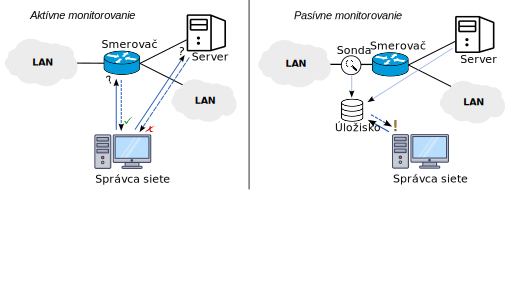
\includegraphics[width=\textwidth]{kapitola_2/aktivne_vs_pasivne_monitorovanie.pdf}
    \caption{Porovnanie spôsobov aktívneho a~pasívneho monitorovania sietí}
    \label{rozdiely_monitorovania}
\end{figure*}

% Architektúra
%  - asi začneš nástřelem architektury - mámě nějakou síť, tu poslouchá sonda a svoje výsledky posílá na kolektor.
%  - zde můžeš popsat i co je to tedy ten tok, který se sleduje, a vůbec proč to tak je... můžeš to např. připodobnit telefonnímu hovoru, který někdy začíná a končí,...
\section{Architektúra NetFlow a~IPFIX}
\label{sec:ipfix_architektura}

Protokol NetFlow, navrhnutý spoločnosťou Cisco v~roku 1996, položil základy monitorovania pomocou sledovania tokov tak, ako ho poznáme dnes \cite{vyvoj_netflow}. Existuje niekoľko
verzií\footnote{Prehľad verzií NetFlow dostupný na: \href{https://ibm.co/3ZD2rve}{ibm.co/3ZD2rve}} tohto protokolu a~medzi jednu z~najstarších a~v~súčasnosti stále používaných sa radí verzia 5, ktorá fixne definuje zbierané údaje
o~tokoch. Od tejto verzie sa odvíjal rad ďalších až po prelomovú 9. verziu, ktorá prešla na dynamický spôsob určovania monitorovaných vlastností pomocou šablón popisujúcich podobu záznamov tokov v~prenášaných správach. Tento mechanizmus dodáva monitorovaniu
flexibilitu a~správy môžu vďaka nemu obsahovať viacero druhov záznamov, ktoré sledujú rozličné atribúty tokov. Protokol IPFIX, popísaný v~sekcii \ref{sec:ipfix}, predstavuje nástupcu NetFlow, ktorý vznikol s~cieľom vytvorenia štandardizovaného spôsobu komunikácie
medzi monitorovacími zariadeniami rôznych výrobcov.

Na obrázku \ref{architektura_ipfix} je zobrazená architektúra využívaná pri monitorovaní sietí pomocou \mbox{NetFlow/IPFIX} \cite{ipfix_architektura}. Proces monitorovania je možné rozdeliť na 3 základné fázy. Prvou z~nich je zachytenie paketov vo~vybraných bodoch siete,
ktoré sú následne analyzované. Zariadenie realizujúce túto činnosť, tiež označované ako \textbf{exportér}, agreguje získané dáta z~paketov v~podobe tokov. Exportérom môže byť ľubovoľný sieťový prvok (napr. smerovač) obohatený o~schopnosť merania tokov, klasický počítač
pripojený do siete s~monitorovacím softvérom alebo špeciálna sieťová sonda. Informácie o~tokoch sú odosielané z~exportéru pomocou príslušného protokolu na zberné miesto zvané \textbf{kolektor}. Druhá fáza popisuje činnosť kolektoru, ktorou je
spracovanie a~úprava dát. Kolektor prijíma správy z~viacerých exportérov, následne môže v~závislosti od jeho konfigurácie toky filtrovať, agregovať, anonymizovať, obohacovať ďalšími informáciami, atď. Upravené záznamy o~tokoch odosiela v~príslušnom formáte na úložisko, alebo
ich priamo poskytuje ostatným aplikáciám k~analýze, ktorá je poslednou fázou procesu monitorovania. Analýza môže prebiehať automatizovane alebo manuálne. Prvý spôsob je vhodný na spracovanie veľkého množstva dát a~najčastejšie sa využíva pri detekcii bezpečnostných anomálií,
má však využitie aj pri tvorení štatistík o~sieti, alebo pri automatizovanom hlásení chýb zariadení. Pri druhom spôsobe správcovia sietí využívajú aplikácie tvoriace vizualizácie nad získanými dátami, ktoré im poskytujú lepší prehľad o~správaní zariadení na sieti.

\begin{figure*}[ht]
    \centering
    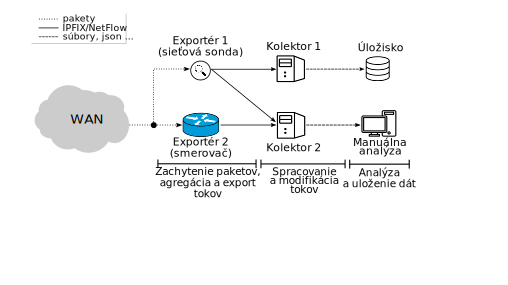
\includegraphics[width=0.9\textwidth]{kapitola_2/architektura.pdf}
    \caption{Príklad monitorovacej architektúry NetFlow/IPFIX \cite{ipfix_architektura}}
    \label{architektura_ipfix}
\end{figure*}

% Sieťový tok
\subsection*{Sieťový tok}
Základným pojmom spojeným s~uvedenými protokolmi je \textbf{tok} (angl. \textit{flow}). Podľa štandardu RFC 7011 \cite{rfc7011} je internetovou komunitou používaných niekoľko definícií tohto pojmu. Samotný štandard definuje sieťový tok následovne:

\begin{quote}
    \textit{Sieťový tok tvorí sada paketov prechádzajúcich pozorovacím bodom počas určitého časového intervalu. Všetky pakety patriace jednému toku obsahujú množinu spoločných vlastností, ktorá ho jednoznačne identifikuje.}
\end{quote}

Sieťový tok obsahuje informácie charakterizujúce komunikáciu zariadení na sieti. Sú tvorené najmä položkami získanými zo sieťových a~transportných hlavičiek paketov, môžu však pochádzať aj z~linkovej či aplikačnej vrstvy. Okrem hodnôt získaných priamo z~paketu
(napr. dĺžka paketu) môže tok obsahovať aj hodnoty z~neho odvodené (napr. číslo autonómneho systému). Množina spoločných vlastností, na základe ktorej sú pakety rozdeľované do príslušných tokov, sa nazýva \textbf{kľúč toku} (angl. \textit{flow key}).
Kľúč si môže každé monitorovacie zariadenie definovať samostatne, najčastejšie sa však používa pätica zložená zo zdrojovej a~cieľovej IP adresy, zdrojového a~cieľového čísla portu a~čísla transportného protokolu.

% Práca IPFIX sondy
%  - další otázka je tedy, co a jak dělá sonda... sonda pasivně poslouchá (není tedy možné její přítomnost zjistit) sbírá data k jednotlivým toků a tím, že si "zparsuje"/zanalyzuje paket,
%       najde v něm klíčové vlastnosti (to je ten klíč toku) a svůj interní záznam si aktualizuje.
%  - co k jednotlivým položkám sbírá? Příklad, možná tabulka? Dělá to každá sonda stejně nebo umí některá více než jiná?
%  - kdy přestane data k danému toku sbírat (timeouty, možnosti vykopnutí FIN flag či přeplnění paměti - mohou to být odrážky, aby se to lépe členilo)
%  - může data zahodit než je někam pošle dle nějakého filtru např. protože to není zájmový provoz?
\subsection*{Činnosť exportéru}

Ako bolo spomenuté v~úvode sekcie \ref{sec:ipfix_architektura}, exportérom môže byť akékoľvek zariadenie pripojené do siete s~možnosťou merania a~exportovania tokov. V~špeciálnom prípade, kedy je exportér dedikovaným zariadením, je označovaný ako sonda.
Hlavnou úlohou sondy je pasívne odpočúvanie komunikácie na sieti, čo dáva správcom siete výhodu, keďže monitorované zariadenia nie sú schopné odhaliť jej prítomnosť. RFC 5470 \cite{rfc5470} rozdeľuje jej činnosť na dva procesy: meranie a~export.

Proces merania začína pozorovaním paketov prechádzajúcich cez rozhranie exportéru. Typicky môže exportér obsahovať viacero rozhraní a~na každom z~nich môže dochádzať ku zberu rozličných dát pomocou samostatných meracích procesov. Vytvorené toky sú však odosielané spoločným
exportným procesom, ktorý znemožňuje presné určenie miesta vytvorenia toku, čo môže byť z~pohľadu správcu siete dôležité k~určeniu pôvodu problému v~sieti. Štandard preto definuje pojem pozorovacej oblasti (angl. \textit{Observation domain}), ktorá identifikuje meracie procesy
v~rámci exportéru. Pozorovacie oblasti sú od seba odlíšené pomocou identifikátoru ODID (\textit{Observation Domain ID}). Štandardom je odporúčané, aby pridelené identifikátory ODID boli spomedzi všetkých zariadení v~danej sieti unikátne, čo umožňuje jednoduché vyhľadanie
exportéru, z~ktorého tok pochádza. Na obrázku \ref{pozorovacia_oblast} je možné vidieť význam zavedenia identifikátoru pozorovacej oblasti konkrétne pri smerovači exportujúcom toky z~viacerých sietí. V~prípade absencie ODID by pre toky odosielané z~tohto zariadenia nebolo
možné jednoznačne určiť ich pôvod.

\begin{figure*}[ht]
    \centering
    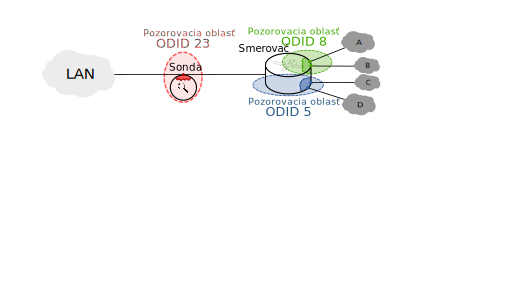
\includegraphics[width=0.9\textwidth]{kapitola_2/pozorovacia_domena.pdf}
    \caption{Príklady pozorovacích oblastí architektúry NetFlow/IPFIX}
    \label{pozorovacia_oblast}
\end{figure*}

Vlastnosti tokov sú udržiavané v~podobe záznamov v~\textbf{medzipamäti tokov} (angl. \textit{flow cache}) \cite{ipfix_architektura}. Proces merania analyzuje pakety prichádzajúce z~bodov pozorovania, pre ktoré sú následne extrahované hodnoty kľúčových vlastností unikátnych pre
daný tok. Na ich základe sa pokúsi sonda o~nájdenie toku v~medzipamäti, s~ktorým následne pracuje. V~prípade, že takýto tok ešte nebol pozorovaný, vytvorí novú položku na jeho popis. Príklad záznamov tokov je možné vidieť na obrázku \ref{meranie_a_export}, ktorý zachytáva
komunikáciu klienta so serverom, kde každý riadok medzipamäte predstavuje jeden tok.

\begin{figure*}[ht]
    \centering
    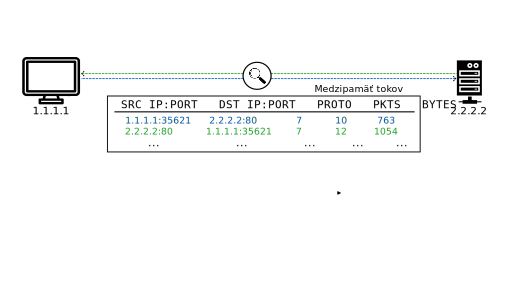
\includegraphics[width=\textwidth]{kapitola_2/export_priklad.pdf}
    \caption{Proces zberu informácií o~tokoch pri komunikácií monitorovaných zariadení}
    \label{meranie_a_export}
\end{figure*}

Štandardom nie je definované, aké informácie sa o~tokoch zbierajú. Existuje však základná a~všeobecne využívaná sada meraných vlastností, ktorá je popísaná v~tabuľke \ref{tab_vlastnosti_tokov}. Táto sada obsahuje atribúty hlavičiek sieťovej a~transportnej vrstvy,
no výrobca exportéru môže často siahnuť aj po atribútoch z~aplikačnej vrstvy, ktoré obsahujú zaujímavejšie informácie z~pohľadu analýzy. Položky záznamov o~tokoch pri technológií IPFIX, popísané pomocou informačných elementov (ich podrobnejší popis sa nachádza v~sekcii
\ref{sec:ipfix}), majú jasne stanovený dátový typ a~sémantiku. Priebežná aktualizácia položiek počas procesu merania je daná agregačnou funkciou, ktorá je špecifická v~závislosti od typu položky \cite{rfc7012}. Je zrejmé, že kľúčové položky definujúce tok nie sú agregované
a~zároveň nemusí existovať agregačná funkcia ani pre niektoré nekľúčové položky. Príkladom takýchto položiek môže byť adresa zisťovaná pri DNS rezolúcii alebo adresa webovej stránky protokolu HTTP. V~takomto prípade nedochádza ku agregácii, ale k~jednorázovému uloženiu
hodnoty skúmanej vlastnosti do toku.

\begin{table}[ht]
    \centering
    \begin{tabular}{ccc}
        \label{tab_vlastnosti_tokov}
        \\ \hline \addlinespace[2pt]
        Sledované vlastnosti & Dátový typ & Agregačná funkcia \\ \hline \addlinespace[1pt]
        \rowcolor{silver} Zdrojová IP adresa & IP adresa & \cellcolor{silver}\\
        \rowcolor{silver} Cieľová IP adresa & IP adresa & \cellcolor{silver}\\
        \rowcolor{silver} Zdrojový port & Nezáporné číslo & \cellcolor{silver}\\
        \rowcolor{silver} Cieľový port & Nezáporné číslo & \cellcolor{silver} \\
        \rowcolor{silver} Protokol & Nezáporné číslo & \multirow{-5}{*}{\cellcolor{silver}\parbox{1.3cm}{Kľúčová \\položka}} \\ \addlinespace[2pt]
        Čas prvého paketu & Dátum & Minimum\\
        Čas posledného paketu & Dátum & Maximum \\
        TCP príznaky & Nezáporné číslo & Bitový OR\\
        Počet bytov & Nezáporné číslo & Suma \\
        Počet paketov & Nezáporné číslo & Suma \\ \bottomrule
    \end{tabular}
    \caption{Prehľad základných informácií o~toku \cite{hutak}}
\end{table}

Druhou časťou funkcie sondy je proces exportu, ktorý rozhoduje o~ukončení a~odoslaní expirovaných tokov. Ich záznamy sú následne odobrané z~medzipamäte tokov a~vložené do novej IPFIX správy, ktorá je odoslaná kolektoru. Tok je odoslaný na export, ak je splnená
jedna z~nasledujúcich podmienok \cite{hutak}:

\begin{itemize}
    \item \textbf{Uplynutie aktívneho časovača}\\
    Aktívny časovač sa používa na pravidelné zisťovanie stavu dlho prebiehajúcich tokov, ktoré môžu vznikať pri prenose väčšieho množstva dát cez sieť. Ak časový úsek, ktorý tok zachytáva, presiahne tento limit, dochádza k~jeho násilnému ukončeniu. Dlho trvajúce toky sú tak
    fragmentované a~odosielané v~podobe kratších tokov. V~prípade absencie tohto časovača by takéto toky boli odoslané na kolektor až po ukončení komunikácie medzi zariadeniami a~správca by nebol priebežne informovaný o~prebiehajúcej komunikácii.
    Limit sa rádovo pohybuje v~jednotkách minút.
    \item \textbf{Uplynutie neaktívneho časovača}\\
    Neaktívny časovač indikuje, že tok nebol určitú dobu aktualizovaný a~má značný význam pri transportných protokoloch, pri ktorých nie je možné detekovať ukončenie komunikácie (napr. UDP).
    Limit sa rádovo pohybuje v~desiatkach sekúnd.
    \item \textbf{Prirodzené ukončenie komunikácie}\\
    Pri niektorých transportných protokoloch (napr. TCP paket s~príznakmi \textit{FIN} alebo \textit{RST}) je možné ukončiť tok, ak došlo ku zisteniu ukončenia spojenia medzi komunikujúcimi zariadeniami.
    \item \textbf{Na základe iných dôvodov}\\
    Do tejto kategórie môže patriť zmena nastavení sondy alebo zaplnenie medzipamäte nad istú úroveň, ktorá by znemožňovala bezproblémové vytváranie nových tokov.
\end{itemize}

Výsledkom činnosti exportéru sú IPFIX správy, ktoré popisujú zachytené toky. Tieto správy sú zasielané na jeden alebo viacero kolektorov pomocou protokolu IPFIX, ktorému sa venuje následujúca sekcia.
\newpage

% Protokol IPFIX
%  - super, uživatel ví, jak se data sbírají a co obsahují... co ale s nimi dále? Na to máme přece protokol NetFlow a IPFIX?
%  - proč máme dva protokoly, co umí? Čím se liší?
%  - dobrá teď známe, co umí... jak je to zákódováno? Šablony? Co položky variabilní délky umí to někdo? Přináší to nějaké komplikace?
%  - ok, máme tedy naformátovaná data, jak se posílají? TCP/UDP/SCTP ok... má to nějaký dopad?
\section{Protokol IPFIX}
\label{sec:ipfix}

Protokol IPFIX je v~súčasnosti štandardizovanou metódou odosielania záznamov o~tokoch z~exportéru na kolektor. Jeho počiatky je možné pozorovať už od roku 2004, kedy pracovná skupina IPFIX\footnote{Prehľad aktivít skupiny:
\href{https://datatracker.ietf.org/group/ipfix/documents}{datatracker.ietf.org/group/ipfix}} (\textit{IP Flow Information Export}), patriaca pod IETF, definovala všeobecné požiadavky monitorovania sietí na základe sledovania tokov a~taktiež analyzovala vhodné protokoly
pre tento proces \cite{rfc5101}. Ako vyplýva z~úvodu sekcie \ref{sec:ipfix_architektura}, \textit{NetFlow v9} bol zvolený za vhodného kandidáta pre vytvorenie nového protokolu, ktorého prvotný návrh bol definovaný v~RFC 5101 začiatkom roku 2008. V~priebehu
nasledujúcich rokov však došlo ku miernym úpravám tejto verzie a~v~roku 2013 sa tieto zmeny premietli do súčasnej podoby IPFIX definovanej v~RFC 7011.

Ako bolo viackrát spomenuté, protokol IPFIX slúži na prenos záznamov o~tokoch z~exportéra na kolektor \cite{rfc7011}. Komunikácia opačným smerom nie je povolená, keďže sa jedná o~jednosmerný protokol. Dôsledkom toho je fakt, že všetky informácie, ktoré kolektor vyžaduje ku dekódovaniu
záznamov, musia byť súčasťou prenášaných správ (výnimkou sú však informačné elementy). Táto vlastnosť napomáha hlavnému cieľu protokolu IPFIX, ktorým je univerzálnosť. Tá umožňuje komunikáciu medzi exportérmi a~kolektormi od rôznych výrobcov, čo je v~praxi častým prípadom.
Záznamy o~tokoch sú v~správach zakódované binárne, pričom dôraz je kladený na priestorovú efektivitu prenášaných dát.

\subsection*{Informačné elementy a~dátové typy}

Definície prenášaných dát sú popísané informačným modelom, ktorý je ustanovený v~RFC 7012 \cite{rfc7012}. Informačný model tvoria \textbf{informačné elementy} slúžiace na popis položiek záznamov o~tokoch nachádzajúcich sa v~IPFIX správach. Definícia informačného
elementu povinne obsahuje názov, identifikačné číslo, popis, dátový typ a~status. Voliteľne môže obsahovať definíciu sémantiky, merané jednotky, rozsah platných hodnôt, atď. Správu informačných elementov zastrešuje organizácia IANA (Internet Assigned Numbers Authority).
Príklady informačných elementov je možné vidieť v~tabuľke \ref{tab_inf_elementy}.

\begin{table}[ht]
    \centering
    \aboverulesep=0ex
    \belowrulesep=0ex
    \renewcommand{\arraystretch}{1.14}
    \begin{tabular}{c|cllp{5.04cm}}
         PEN & ID &  Názov & Dátový typ & Popis \\ \toprule
         \multirow{4}{*}{0} & 2 & packetDeltaCount & unsigned64 & Počet prenesených paketov \\
         & 8 & sourceIPv4Address & ipv4Address & Zdrojová IPv4 adresa \\
         & 11 & destinationTransportPort & unsigned16 & Cieľové číslo portu \\
         & 80 & destinationMacAddress & macAddress & Cieľová MAC adresa \\ \midrule
         \multirow{2}{*}{6876\footnotemark} & 166 & smtpSubject & string & Subjekt emailovej správy  \\
         & 553 & certToolId & unsigned32 & Identifikátor CERT zariadenia  \\ \midrule
         5915\footnotemark & 890 & ingressInterfaceAttr & unsigned64 & Port pripojeného virtuálneho zariadenia
    \end{tabular}
    \caption{Časti definícií vybraných informačných elementov}
    \label{tab_inf_elementy}
\end{table}

\footnotetext[3]{Registrované entity privátneho rozsahu CERT: \href{https://tools.netsa.cert.org/cert-ipfix-registry/}{tools.netsa.cert.org/cert-ipfix-registry}}
\footnotetext[4]{Registrované entity privátneho rozsahu VMware (skrátený odkaz): \href{https://docs.vmware.com/en/VMware-NSX-Data-Center-for-vSphere/6.4/com.vmware.nsx.admin.doc/GUID-40805D0E-8A97-4011-B85C-CBF37812DBB5.html}{bit.ly/3yrBFtF}}

Samotné informačné elementy taktiež podliehali zmenám spolu s~protokolom IPFIX. Pôvodný návrh informačného modelu v~RFC 5102 \cite{rfc5102} definoval základnú množinu všeobecne sledovaných vlastností o~tokoch naprieč rôznymi výrobcami, ktorá bola neskôr (v~RFC 7012) presunutá
do \textbf{spoločného rozsahu}\footnote{Prehľad aktuálne platných informačných elementov: \href{https://www.iana.org/assignments/ipfix/ipfix.xhtml}{www.iana.org/assignments/ipfix}} definícií nového modelu. Keďže pridávanie nových definícií do tohto rozsahu podlieha štandardizovanému procesu,
výrobcovia exportérov môžu požiadať o~pridelenie \textbf{privátneho rozsahu}\footnote[6]{Zoznam registrovaných privátnych domén: \\ \href{https://www.iana.org/assignments/enterprise-numbers/enterprise-numbers}
{www.iana.org/assignments/enterprise-numbers/enterprise-numbers}}. Privátny rozsah je identifikovaný pomocou čísla PEN (Private Enterprise Number) a~obsahuje definície informačných elementov, ktoré sú špecifické pre daného výrobcu, alebo majú experimentálny charakter.
Pre štandardne definované informačné elementy pod správou organizácie IANA je vyhradený privátny rozsah s~identifikačným číslom PEN 0.

\subsection*{Štruktúra IPFIX správy}

\begin{figure*}[ht]
    \centering
    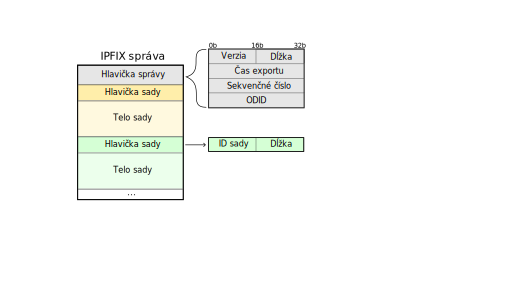
\includegraphics[width=0.6\textwidth]{kapitola_2/ipfix_struktura.pdf}
    \caption{Štruktúra IPFIX správy}
    \label{ipfix_struktura}
\end{figure*}

Popis IPFIX správy vychádza z~jej definície v~RFC 7011 \cite{rfc7011}. Štruktúra správy, ktorú je možné vidieť na obrázku \ref{ipfix_struktura}, začína povinnou hlavičkou, za ktorou voliteľne nasledujú definície sád obsahujúce dáta rôzneho charakteru v~závislosti od ich typu.
Na začiatku hlavičky správy je zakódovaná verzia použitého protokolu.
Pre \mbox{IPFIX} je táto hodnota 10, pri iných verziách (NetFlow) predstavuje číslo použitého protokolu. Nasleduje dĺžka celej správy (vrátane hlavičky), čas exportu, sekvenčné číslo a~identifikátor pozorovacej domény (ODID). Na kódovanie dát správy sa používa
\textit{network byte order} (alebo takzvaný \textit{big-endian}) a~zariadenia využívajúce inú endianitu musia pri práci s~dátami využívať konvertovacie funkcie.

Za hlavičkou samotnej IPFIX správy nasledujú jednotlivé sady, kde každá je zložená z~hlavičky a~tela. Hlavička sady obsahuje identifikačné číslo spolu s~celkovou dĺžkou sady, ktorú definuje.
V~závislosti od typu sady je odvodená hodnota identifikačného čísla a~obsah tela sady. Existujú 3 typy sád, a~to sady šablón záznamov o~tokoch (angl. \textit{Template Set}), sady šablón nastavení a~prevádzkových parametrov exportéru
(angl. \textit{Option Template Set}) a~dátové sady (angl. \textit{Data Set}).

Šablónové sady obsahujú definície \textbf{šablón}, ktoré sú dôležitým mechanizmom IPFIX správ. Šablóny popisujú štruktúru prenášaných dátových záznamov tokov alebo prevádzkových parameterov. K~určeniu položiek, z~ktorých je dátový záznam zložený, sa používajú spomínané
informačné elementy, ktoré popisujú význam jednotlivých polí (napr. zdrojová IP adresa, počet prenesených bajtov, atď.). Príklad štruktúry šablóny je na obrázku \ref{ipfix_sablona}. Každá šablóna začína identifikačným číslom, ktoré je z~intervalu hodnôt <\,$256-65535$\,>,
za ktorým sa nachádza počet položiek šablóny. Ďalej nasleduje usporiadaná sekvencia definícií položiek toku, ktoré sú primárne zložené z~identifikačného čísla informačného elementu a~maximálnej veľkosti daného poľa. Ak pochádza informačný element z~privátneho rozsahu, najvyšší
bit identifikátora elementu je nastavený na jednotku a~definícia je rozšírená o~číslo PEN.

\begin{figure*}[ht]
    \centering
    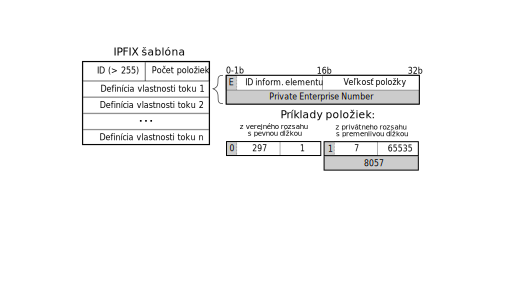
\includegraphics[width=0.9\textwidth]{kapitola_2/ipfix_sablona.pdf}
    \caption{Štruktúra IPFIX šablóny}
    \label{ipfix_sablona}
\end{figure*}

Pozorný čitateľ si mohol všimnúť, že samotný informačný element definuje dátový typ, ktorým udáva veľkosť sledovanej vlastnosti. Prečo sa teda nachádza veľkosť aj v~položke šablóny? Prvým dôvodom je fakt, že exportér nemusí striktne použiť veľkosť dátového
typu a~môže sa rozhodnúť zakódovať dáta v~menšej veľkosti, ktorá je uložená do položky šablóny. Druhý dôvod súvisí so zakódovaním textových reťazcov, ktoré majú \textbf{premenlivú dĺžku}. Pevne definovaná veľkosť by predstavovala ich skrátenie alebo v~opačnom prípade
plytvanie pamäte. Z~toho dôvodu majú položky s~variabilnou dĺžkou zakódovanú ich skutočnú veľkosť v~prefixe dátového záznamu a~veľkosť v~definícii šablóny obsahuje rezervovanú hodnotu 65535, ktorá je vyhradená pre položky s~dynamickou veľkosťou.

Sady šablón sa delia na dve skupiny. Prvou z~nich sú vyššie spomenuté \textit{sady šablón záznamov o~tokoch}, ktoré výhradne popisujú monitorované toky. Takýto typ sady je definovaný identifikačným číslom 2 v~hlavičke sady. Druhým typom sú \textit{sady šablón nastavení
a~prevádzkových parametrov exportéru}, ktoré popisujú parametre monitorovania a~sú identifikované číslom 3 v~hlavičke sady. Šablóny tohto typu sú navyše rozšírené o~definíciu políčok určujúcich kontext záznamu.

\textbf{Dátová sada} je zložená z~dátových záznamov obsahujúcich položky tokov. Identifikačné číslo dátovej sady nadobúda hodnoty od 256 a~spája sadu so šablónou, ktorá ju popisuje. Dátové záznamy môžu byť statické, ak obsahujú výhradne položky s~fixne danou veľkosťou,
alebo dynamické, ak obsahujú aspoň jednu položku s~premenlivou veľkosťou. Práca s~dynamickými záznamami môže prinášať rôzne úskalia, keďže dĺžku takého záznamu nie je možné určiť z~definície šablóny. Tieto okolnosti často vedú k~potrebe manuálnej iterácie všetkých položiek,
s~cieľom určenia začiatku nového záznamu. Položky dynamických záznamov s~premenlivou veľkosťou obsahujú prefix ich skutočnej dĺžky, ktorý je jedno-bajtový v~prípade, že je jeho veľkosť menšia ako hodnota 255. V~opačnom prípade je hodnota prvého bajtu 0xFF a~veľkosť položky
je zakódovaná v~následujúcich dvoch bajtoch (maximálna veľkosť je teda 65535). Príklad dátových záznamov a~ich prepojenia so~šablónami je popísaný na obrázku \ref{ipfix_priklad}.

\begin{figure*}[ht]
    \centering
    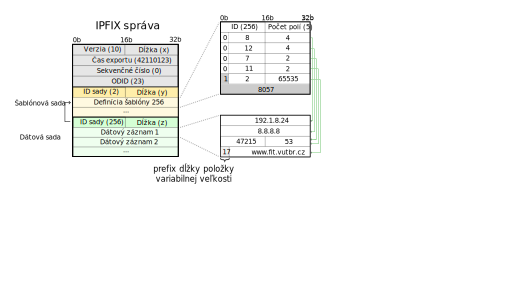
\includegraphics[width=\textwidth]{kapitola_2/ipfix_priklad.pdf}
    \caption{Príklad IPFIX správy s~prepojením dátového záznamu na šablónu}
    \label{ipfix_priklad}
\end{figure*}


% Práca IPFIX kolektoru
%  - Na druhé straně je kolektor? Může se nějak pobavit se sondou či ji nakonfigurovat? Nemůže, neboť je NetFlow/IPFIX protokol jednosměrný...
%  - Dobře, co tedy kolektor dělá? Musí si držet šablony pro danou komunikaci, aby rozumněl posílaným záznamům? Může se stát, že některým položkám nerozumí? Zná jejich datový typ? Přenáší to NetFlow/IPFIX protokol? Ne? Tak jak to řeší...
%  - Co s daty, které interpretuje dělá? Filtruje, anonymizuje, modifikuje?
%  - a pak? Přeposílá dále, konvertuje do jiného formátu? Nebo ukládá do souboru pro pozdější zpracování?
\section{Popis práce kolektoru}
\label{sec:collector_overview}

Poslednou sekciou tejto kapitoly je priblíženie práce kolektoru, ktorá začína nadviazaním spojenia s~niekoľkými exportérmi a~pokračuje prijímaním generovaných správ \cite{rfc5153}. Pri odosielaní tokov z~exportéru sa za účelom zníženia množstva prenesených dát
nemusia v~každej IPFIX správe vyskytovať definície šablón. Spravidla sú odosielané ihneď po vytvorení spojenia s~kolektorom. Následujúce správy môžu obsahovať dátové sady, ktoré sa odkazujú na tieto šablóny. Tento fakt udáva jednu z~činností kolektoru, ktorou je udržiavanie
odkazov na doposiaľ prijaté šablóny. Okrem definícií šablón môžu správy obsahovať aj záznamy o~zrušení šablón (angl. \textit{Template Withdrawal}) alebo o~ich aktualizácii, na ktoré musí byť kolektor schopný reagovať.

\subsection*{Vplyv transportných protokolov na správu šablón}

Udržiavanie odkazov na šablóny úzko súvisí s~typom transportného protokolu použitého k~prenosu správ z~exportéru na kolektor. Najjednoduchším prípadom je použite protokolu \textbf{TCP}, ktorý zabezpečuje spoľahlivé doručenie správ v~správnom poradí. Pre protokoly
SCTP alebo UDP je štandardom \cite{rfc5153} mierne upravený proces odosielania IPFIX správ. Protokol \textbf{SCTP}, ktorý spája vlastnosti TCP a~UDP, kombinuje prístupy zaručeného a~nezaručeného odosielania správ. Z~toho vyplýva podmienka, že všetky IPFIX správy obsahujúce
definíciu alebo odstránenie šablóny, musia byť spoľahlivo odoslané so zachovaním poradia doručenia. Správy obsahujúce dátové záznamy môžu, no nemusia byť odosielané týmto spôsobom.

V~prípade \textbf{UDP} je situácia zložitejšia, keďže doručenie správ nie je garantované. Prvým problémom spojeným s~týmto protokolom je možná strata paketov obsahujúcich definície šablón. V~takom prípade by kolektor nebol schopný interpretovať prichádzajúce dátové záznamy,
čo by predstavovalo výpadok informácií o~stave siete. Čiastočné riešenie sa ponúka zo strany exportéru v~podobe pravidelného odosielania používaných šablón v~určitých časových intervaloch. Periodické odosielanie použitých šablón tak zvyšuje šance ich úspešného doručenia na kolektor.
Ďalším problémom je možné doručenie správ v~nesprávnom poradí, kedy oneskorené správy s~dátovými záznamami môžu používať šablóny, ktoré boli medzičasom redefinované. V~takom prípade by mohol kolektor mylne interpretovať dátové záznamy, čo by následne mohlo viesť ku chybám vo výsledných dát.

Kolektor musí byť ďalej schopný rozlíšiť pôvod získaných záznamov, ktorý je spojený s~\textbf{kontextom platnosti šablóny} \cite{hutak}. Keďže zvyčajne sú správy na kolektor odosielané z~rôznych exportérov, je zrejmé, že každý z~nich môže definovať rôzne šablóny popisujúce monitorované
vlastnosti. Rovnaké identifikačné čísla šablón však môžu byť súčasne využívané viacerými exportérmi odosielajúcimi správy na kolektor v~rovnakom čase. Ak exportér navyše obsahuje viacero pozorovacích domén, unikátnosť identifikátoru šablóny je zabezpečená iba v~rámci domény, z~ktorej pochádza.
Kolektor musí s~týmito situáciami počítať aby bol schopný úspešne interpretovať správy prijaté z~rôznych exportérov, alebo z~rôznych pozorovacích oblastí jedného exportéru.
Z~toho vyplýva, že kontext platnosti šablóny je viazaný na kombináciu transportného spojenia s~daným exportérom a~identifikátorom pozorovacej domény (ODID) šablóny.

\subsection*{Správa informačných elementov}

Pre dekódovanie dátových záznamov sa vyžaduje znalosť príslušných informačných elementov, ktoré nie sú prenášané použitým protokolom. V~prípade, že kolektor nemá k~dispozícii tieto definície, nedokáže pracovať s~dátovými záznamami, preto ich následne ignoruje alebo zahodí \cite{rfc5153}.
Z~toho dôvodu je od kolektoru prinajmenšom očakávaná znalosť elementov zo spoločného rozsahu. V~ideálnom prípade by však mal podporovať možnosť dynamického doplnenia databázy informačných elementov o~definície prvkov z~privátnych rozsahov.

\subsection*{Práca s~dátovými záznamami}

Kolektor má po úspešnom prijatí a~interpretácií správ možnosť pracovať s~dátami, ktoré z~nich boli získané. Medzi často využívané funkcie pri práci s~prichádzajúcimi tokmi patrí ich \textbf{filtrovanie}. V~závislosti od nasadenia kolektoru môže byť žiadúce, aby spracovával iba
určitú časť záznamov spĺňajúcich podmienku danú filtračným výrazom. Filtrovaním tak dochádza k~zníženiu záťaže potrebnej na spracovanie správ a~zároveň k~umožneniu rozdelenia monitorovania väčších sietí na menšie úseky.
Ak kolektor navyše prijíma správy z~viacerých exportérov, môže získané dáta ďalej agregovať, čím znižuje nároky potrebné na ich uskladnenie. \textbf{Profilovanie} tokov je nemenej využívaným prostriedkom, ktorý klasifikuje prijaté toky na základe vopred definovaných kritérií.
Najčastejším prípadom profilovania je kategorizácia tokov podľa použitého protokolu, čo poskytuje správcom informáciu o~najpoužívanejších službách v~sieti. Nezvyčajný nárast výskytu služby tak môže predstavovať bezpečnostné riziko, napríklad zvýšenie počtu TCP paketov s~príznakom SYN je
najčastejším indikátorom SYN-flood\footnote{SYN-flood alebo záplava SYN paketov je forma DoS (\textit{Denial of Service}) útoku, pri ktorej útočník čiastočne nadviaže spojenie s~cieľovým zariadením a~neumožňuje jeho využívanie inými užívateľmi} útoku \cite{wiki:SYN_flood}.

Niektoré analyticky zaujímavé atribúty popisujúce toky nemusia byť nevyhnutne súčasťou exportovaných správ, ako bolo spomenuté v~úvodnej kapitole. Jedným z~dôvodov ich absencie môžu byť napríklad limitované prostriedky exportéru alebo veľké množstvo času spojené s~ich získaním.
V~prípade, že je exportér nasadený na hlavných internetových linkách, musí byť každú sekundu schopný spracovať až státisíce paketov. Z~toho dôvodu by získavanie informácií z~tretích strán predstavovalo časovo kritické úseky práce exportéru, ktoré
by mali dopad na jeho výkonnosť. Obohacovanie tokov preto často spadá na kolektory, ktoré pracujú už s~vopred agregovanými dátami. Súčasným trendom v~tejto oblasti je navyše použitie distribuovanej architektúry \cite{distribuovana_architektura}, ktorá je založená na rozložení
spracovania tokov medzi pracovné uzly (skupinu kolektorov), čo umožňuje zvýšenie škálovateľnosti architektúry pri monitorovaní rozsiahlejších sietí.

\subsection*{Formát výstupných dát}

Modifikované záznamy sú následne odosielané v~rôznych formátoch na úložisko, alebo sú poskytované ďalším aplikáciám k~analýze. Formáty podporované kolektorom závisia od jeho implementácie a~zároveň aj od aplikácií pracujúcich nad týmito dátami. Príklady konkrétnych kolektorov
a~nimi podporovaných formátov sú popísané v~práci: \textit{Practical Experience with IPFIX Flow Collectors} \cite{velan_kolektory}. Rada súčasných kolektorov podporuje export záznamov v~databázových formátoch ako je MySQL alebo FastBit, ktoré je možné vidieť pri kolektoroch
\textit{nProbe} alebo \textit{Vermont}. Ďalšou populárnou možnosťou je použitie binárnych súborov, pri ktorých si väčšina kolektorov definuje vlastný spôsob ukladania dát. Príkladom kolektorov využívajúcich binárne súbory sú \textit{SiLK}, \textit{nfcapd} alebo \textit{IPFIXcol2}
(využívajúci binárny formát FDS). Väčšina kolektorov podporuje okrem spomínaných spôsobov aj možnosť uloženia záznamov vo formátoch JSON alebo v~textovej podobe.

\subsection*{Analýza dát}

Existuje veľké množstvo aplikácií poskytujúcich analýzu získaných informácií. Jednou z~najznámejších je sada nástrojov \textit{nfdump}\footnote{Stránky nástroja nfdump: \href{https://github.com/phaag/nfdump}{github.com/phaag/nfdump}}, ktorá obsahuje softvérový
exportér a~kolektor spolu s~rozšíreniami ako je filtrovanie, profilovanie a~obohacovanie tokov. Nevýhodou práce s~týmto nástrojom je jeho nastavenie a~limitovaná vizualizácia dát, ktoré sú realizované prostredníctvom príkazového riadku. Tieto nevýhody sú však kompenzované
nadstavbami, ktoré umožňujú užívateľom získané informácie integrovať s~inými aplikáciami poskytujúcimi vizualizáciu dát.
Pokročilejšími nástrojmi sú \textit{NfSen}\footnote{Stránky nástroja NfSen: \href{https://nfsen.sourceforge.net}{nfsen.sourceforge.net}}, ktorý poskytuje
základné webové rozhranie pre grafické zobrazovanie informácií o~tokoch alebo \textit{NEMEA}\footnote{Stránky nástroja NEMEA: \href{https://github.com/CESNET/Nemea}{github.com/CESNET/Nemea}} predstavujúca ľahko rozšíriteľný nástroj pre určovanie rôznych druhov útokov.
Nástroje ako \textit{ntop}\footnote{Stránky nástroja ntop: \href{https://www.ntop.org}{ntop.org}} alebo \textit{Flowmon}\footnote{Stránky nástroja Flowmon: \href{https://www.flowmon.com}{flowmon.com}}, ktoré spájajú prvky detekcie útokov, správy sietí a~pokročilej vizualizácie,
sa vyskytujú v~popredí nástrojov používaných na správu sietí.

% -------------------------------------------  POPIS KOLEKTORU ------------------------------------------- %
% plánovaný rozsah: spolu s popisom monitorovania 40-50% práce => cca 16-20 strán pri 40 stranách celej práce
% poznámky: popisať kolektor celkovo (ale v skratke) => nevenovať sa veľmi detailom

\chapter{Analýza kolektoru IPFIXcol2}
\label{chpt:kolektor}

Kolektorov určených k~zberu monitorovacích dát je v~dnešnej dobe veľké množstvo, pričom každý z~nich poskytuje iné možnosti práce s~dátami. Jedným z~verejne vyvíjaných je kolektor IPFIXcol\footnote{Odkaz na stránky kolektoru IPFIXcol:
\href{https://www.liberouter.org/technologies/ipfixcol/}{liberouter.org/technologies/ipfixcol}}, vytvorený tímom liberouter\footnote{Odkaz na stránky tímu liberouter: \href{https://www.liberouter.org}{liberouter.org}} patriacim pod združenie CESNET. Počiatky vývoja tohto kolektoru
siahajú do roku 2012, teda do obdobia vzniku jeho prvej verzie \cite{ipfixcol}. V~priebehu jeho používania sa však vyskytli problémy spojené s~jeho návrhom a~udržiavaním, ktoré vyústili do vytvorenia novej verzie kolektoru pod názvom
IPFIXcol2\footnote{Odkaz na stránky kolektoru IPFIXcol2: \href{https://github.com/CESNET/ipfixcol2}{github.com/CESNET/ipfixcol2}} v~roku 2017, ktorému sa venujú nasledujúce časti tejto práce. Cieľom nasledujúcej kapitoly je priblíženie jednotlivých častí kolektoru IPFIXcol2,
počínajúc popisom jeho architektúry, pokračujúc prehľadom jadra kolektoru a~správy šablón, končiac sekciou o~používaných moduloch. Poznatky o~tomto kolektore vychádzajú z~diplomovej práce jedného z~jeho hlavných vývojárov Ing. Lukáša Hutáka s~názvom \textit{Nová generace IPFIX kolektoru}~\cite{hutak}.

\section{Prehľad architektúry}
\label{sec:ipfixcol2_zaklad}

Počas tvorby kolektoru IPFIXcol2 bola zvláštna pozornosť venovaná jeho vlastnostiam, ako sú flexibilita a~vysoká rýchlosť spracovania. Táto zvýšená pozornosť sa premietla v~návrhu jeho architektúry. Jej základným prvkom je \textbf{zreťazená linka}, po ktorej prijaté správy putujú cez kolektor.
Na tejto zreťazenej linke sa nachádzajú \textbf{moduly} vykonávajúce hlavné funkcie kolektoru, ktorými sú nadviazanie spojenia s~exportérom, prijatie správ, správa šablón, modifikácia záznamov a~pod. Modularita poskytuje užívateľom možnosť nastavenia kolektoru podľa ich potrieb,
zároveň umožňuje tieto nastavenia kedykoľvek zmeniť. K~popisu konfigurácie sa používa jazyk XML, pomocou ktorého je súčasne možné pridávať definície informačných elementov. Práca s~modulmi ďalej ponúka možnosti zvyšovania výkonnosti pomocou
\textbf{paralelizácie}, pretože je práca každej inštancie modulu vykonávaná v~separátných vláknách.

Architektúra kolektoru, zobrazená na obrázku \ref{ipfixcol2_architektura}, definuje tri druhy modulov: vstupné, vnútorné a~výstupné. Úlohou vstupných modulov je získavanie IPFIX správ, ktoré môže byť realizované komunikáciou s~exportérom pomocou príslušného protokolu alebo iného zdroja dát
(napr. súborov). Každý vstupný modul je spojený s~preprocesorom, ktorý je bližšie popísaný v~sekcii \ref{sec:ipfixcol2_jadro}. Pre začiatok stačí uviesť, že preprocesor slúži na kontrolu prichádzajúcich správ a~správu prijatých šablón. Správy sú prenášané zreťazenou linkou ku vnútorným modulom
realizujúcim činnosti spojené s~úpravou záznamov o~tokoch, akými sú napríklad anonymizácia, filtrovanie a~profilovanie. Ďalej smerujú na výstupný manažér, ktorý preposiela ich kópie jednotlivým výstupným modulom. Výstupné moduly konvertujú prijaté správy do príslušného formátu a~odosielajú na
úložisko, alebo ich poskytujú ďalším aplikáciám. Z~popisu architektúry vyplýva, že zásuvné moduly sa špecializujú na určité časti práce kolektoru, zatiaľ čo správu týchto modulov, do ktorej patrí ich prepojenie a~vzájomná komunikácia, realizuje \textbf{jadro} kolektoru.

\begin{figure}[ht]
    \centering
    \includegraphics[width=\textwidth]{kapitola_3/ipfixcol2_architektura.pdf}
    \caption{Architektúra kolektoru IPFIXcol2 \cite{hutak}}
    \label{ipfixcol2_architektura}
\end{figure}

\section{Popis činnosti jadra kolektoru}
\label{sec:ipfixcol2_jadro}

Medzi základné činnosti jadra patrí konfigurácia kolektoru, vytváranie inštancií jednotlivých modulov a~zabezpečovanie komunikácie medzi nimi, ktorá je realizovaná prenášaním správ pomocou zreťazenej linky. V~rámci tejto komunikácie existujú štyri
typy správ, ktoré sa v~kolektore vyskytujú.

\subsection*{Dátová správa}

Najčastejšie prenášanými správami v~kolektore IPFIXcol2 sú dátové správy, ktorých úlohou je udržiavať informácie o~surových Netflow/IPFIX správach. Tieto informácie sú uložené v~takzvanej obálke, ktorú je možné vidieť na obrázku \ref{datova_sprava}. Dátové správy vznikajú
vo vstupných moduloch, ktoré do obálky vložia odkaz na surovú správu spolu s~jej dĺžkou a~kontextom. Kontext správy obsahuje údaje o~spojení s~exportérom a~ODID, z~ktorého informácie o~tokoch pochádzajú. Na základe znalosti pôvodu správy je možné určiť šablóny
definované týmto zdrojom, ktoré sú následne použité na interpretáciu dátových záznamov. Vytvorená dátová správa je odoslaná preprocesoru na ďalšie spracovanie.

Činnosť \textbf{preprocesora} začína určením verzie použitého protokolu z~prijatej správy (Net\-Flow v5/v9, IPFIX). Pre správy typu Neflow navyše prebieha aj konvertovanie do IPFIX podoby, čo umožňuje kolektoru spracovávať správy v~rôznych formátoch univerzálnym spôsobom.
Preprocesor následne identifikuje všetky sady vyskyujúce sa v~IPFIX správe. Odkazy na začiatky týchto sád sú doplnené do obálky dátovej správy. V~prípade, že preprocesor narazí na šablónovú sadu, extrahuje z~nej definície šablón. Udržiavanie doposiaľ videných
šablón prebieha v~manažéri šablón, ktorý je bližšie popísaný v~sekcii \ref{sec:ipfixcol2_sablony}. V~závislosti od typu definície šablóny (vytvorenie, odstránenie, redefinícia) je aktualizovaný stav manažéra. Pri dátových sadách je pre každý záznam vytvorená položka v~obálke
dátovej správy obsahujúca informácie o~danom zázname. Tieto položky (taktiež zobrazené na obrázku \ref{datova_sprava}) predstavujú kľúčovú časť práce s~dátovými správami. Patria k~nim:

\begin{itemize}
    \setlength\itemsep{-0.5em}
    \item \textit{ukazovateľ na pozíciu záznamu v~surovej správe} -- používa sa na zistenie hodnoty položiek dátového záznamu
    \item \textit{skutočná dĺžka záznamu} -- v~prípade pevnej dĺžky záznamu je zistená z~definície šablóny, v~opačnom prípade preprocesor odvodí dĺžku z~prefixov dynamických záznamov
    \item \textit{odkaz na šablónu záznamu} -- šablóna popisujúca záznam je uložená v~manažéri šablón
    \item \textit{snímka šablón} -- stav manažéra šablón v~čase prijatia šablóny (popísaný v~sekcii \ref{sec:ipfixcol2_sablony})
\end{itemize}

\begin{figure}[ht]
    \centering
    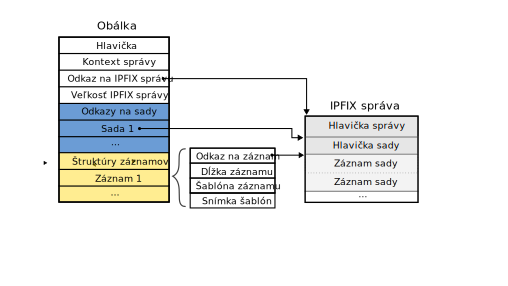
\includegraphics[width=0.8\textwidth]{kapitola_3/datova_sprava.pdf}
    \caption{Obálka správy spolu so~štruktúrou dátového záznamu}
    \label{datova_sprava}
\end{figure}

Význam ukladania týchto informácií spočíva v~zjednodušení manipulácie s~IPFIX správami počas práce vykonávanej ďalšími modulmi kolektoru. Väčšina informácií, ktoré moduly potrebujú ku~svojej činnosti, sa nachádza priamo v~obálke dátovej správy, a~preto je potreba siahnuť po
surovej správe minimálna. Navyše tým dochádza ku zlepšeniu výkonu kolektoru, keďže iterácia cez položky surovej správy prebieha jednorázovo v~preprocesore a~nie separátne v~každom module.

\subsection*{Správa sedenia}
Ďalším druhom správ vyskytujúcich sa v~kolektore IPFIXcol2 sú správy sedenia (angl. \textit{session message}), ktorých úlohou je poskytovať informácie o~zmene stavu transportného spojenia s~exportérom. Štruktúra tejto správy je zložená z~identifikátoru sedenia a~typu udalosti,
ktorým môže byť nadviazanie alebo ukončenie spojenia. Správy sedenia vznikajú primárne vo vstupných moduloch, zároveň však môžu byť vytvorené počas činnosti preprocesoru. V~prípade, že preprocesor detekuje chybu pri spracovaní prijatej správy, môže uzatvoriť spojenie, z~ktorého správa pochádza,
pričom je zároveň vygenerovaná nová správa sedenia popisujúca uzatvorenie tohto spojenia. Význam tohto typu správ je viditeľný pri správe šablón, kedy prijatie správy o~ukončení sedenia preprocesorom značí, že šablóny, ktoré boli definované v~tomto spojení už nebudú používané,
a~teda môžu byť odstránené.

\subsection*{Odpadová správa}

Nemenej využívaným typom správ sú odpadové správy (angl. \textit{garbage message}), ktoré zabezpečujú korektné uvoľňovanie pamäte pre objekty spravované kolektorom. Ich využitie je najlepšie demonštrované na nasledujúcom príklade. Predstavme si situáciu zobrazenú na obrázku
\ref{odpadova_sprava_1}, kedy kolektor prijme správu o~zrušení transportného sedenia s~exportérom. Zároveň sa v~zreťazenej linke môže nachádzať prijatá, ale doposiaľ nespracovaná dátová správa obsahujúca záznamy, ktoré sa odkazujú na šablóny definované v~tomto spojení.
V~takom prípade by preprocesor nemohol uvoľniť šablóny vo svojom manažéri, keďže sú ešte stále odkazované dátovou správou.

\begin{figure}[ht]
    \includegraphics[width=0.8\textwidth]{kapitola_3/odpadova_sprava_1.pdf}
    \caption{Príklad dátovej správy obsahujúcej záznamy odkazujúce na aktívne šablóny v~manažéri}
    \label{odpadova_sprava_1}
\end{figure}

Jedným z~možných riešení je uložiť použité šablóny do odpadovej správy, ktorá je odoslaná do zreťazenej linky. Odpadová správa, ktorá je zobrazená na obrázku \ref{odpadova_sprava_2}, obsahuje odkaz na rušený objekt spolu s~funkciou, ktorá sa použije na jeho odstránenie.
Dôležitou vlastnosťou využívanou pri odpadovej správe je zachovanie poradia odosielaných správ v~zreťazenej linke kolektoru. Táto vlastnosť garantuje, že všetky dátové správy odkazujúce sa na rušené šablóny boli spracované skôr, než sa odpadová správa dostane na koniec zreťazenej linky.
Na základe týchto okolností je možné objekt odpadovej správy na výstupných moduloch jednoducho odstrániť.

\begin{figure}[ht]
    \centering
    \includegraphics[width=0.6\textwidth]{kapitola_3/odpadova_sprava_2.pdf}
    \caption{Použitie odpadovej správy na odstránenie šablón}
    \label{odpadova_sprava_2}
\end{figure}

\subsection*{Terminačná správa}
Posledným typom správy je tzv. terminačná správa, ktorá je de facto poslednou prechádzajúcou kolektorom. Prijatie terminačnej správy modulom oznamuje ukončenie činnosti kolektoru, ktoré je spojené s~uvoľňovaním alokovaných zdrojov a~ukončením práce modulov.

\section{Správa šablón}
\label{sec:ipfixcol2_sablony}

Správa šablón je realizovaná preprocesorom, ktorý z~prijatých správ extrahuje definície šablón. Informácie o~šablónach definície následne ukladá do vnútornej štruktúry používanej v~kolektore IPFIXcol2, ktorú je možné vidieť na obrázku \ref{ipfixcol2_sablona}. Štruktúra
šablóny obsahuje základné informácie, ako napríklad jej typ (šablóna dátových záznamov alebo prevádzkových parametrov), ID šablóny, dĺžku a~odkaz na surovú šablónu. Časové značky popisujú, kedy bola šablóna prvýkrát definovaná, kedy bola naposledy obnovená alebo, v~prípade
protokolu UDP, v~akom čase dôjde ku vypršaniu jej platnosti. Štruktúra je ukončená zoznamom položiek, ktoré šablóna definuje.

\begin{figure}[ht]
    \centering
    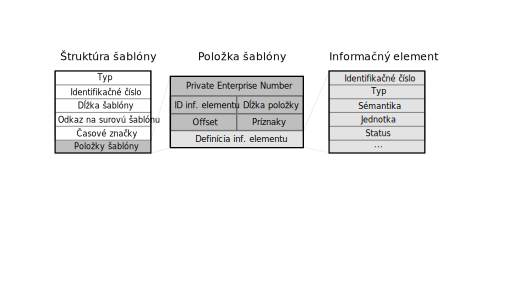
\includegraphics[width=\textwidth]{kapitola_3/ipfixcol2_sablona.pdf}
    \caption{Spôsob uloženia informácií o~šablóne kolektoru IPFIXcol2}
    \label{ipfixcol2_sablona}
\end{figure}

Štruktúra položky šablóny je okrem základných informácií definovaných štandardom (obrázok \ref{ipfix_sablona}) obohatená o~políčka \textit{offsetu} alebo príznakov položky. Offset udáva polohu danej položky od začiatku šablóny a~príznaky určujú dodatočné informácie
(napr. viacnásobný alebo posledný výskyt, kľúčová položka, atď). Položka šablóny tiež zahrňuje odkaz na príslušný informačný element, ktorý ju popisuje. Informačné elementy sú v~kolektore spravované manažérom informačných elementov, ktorý po spustení kolektoru získa definície elementov
zo zvoleného konfiguračného súboru.

Šablóny sú uchovávané v~\textbf{manažérovi šablón}, ktorý poskytuje fundamentálne operácie na prácu so šablónami, akými sú vkladanie, mazanie alebo vyhľadávanie na základe identifikačného čísla. Z~dôvodu obmedzeného počtu definícií šablón, ktorý vychádza z~pevne stanoveného rozsahu
identifikačných čísel, je možné ich uloženie v~dvojúrovňovej adresovacej tabuľke. Prvá úroveň tejto tabuľky rozdeľuje množinu všetkých identifikačných čísel na rovnako veľké intervaly, ktoré obsahujú v~druhej úrovni zoznam definícií šablón. Tento spôsob uloženia je možné
vidieť na obrázku \ref{ipfixcol2_snimky}. Kolektor IPFIXcol2 navyše adresuje problémy správy šablón spojené s~ich redefinovaním alebo spracovaním oneskorených správ.

Pri zmene definície šablóny sa v~zreťazenej linke môžu nachádzať dátové správy, ktorých záznamy boli popísané pomocou pôvodnej šablóny. Druhým problémom je interpretácia oneskorených správ, ktorých záznamy sa môžu odkazovať na medzičasom zmenené šablóny.
Riešenie, ktorým manažér šablón disponuje, je prepájanie definícií šablón s~časom ich vytvorenia. Tento proces je realizovaný pomocou \textbf{snímok šablón} (angl. \textit{snapshots}). K~ich vytváraniu dochádza pri zmene definície šablóny, pričom ostáva k~dispozícii aj pôvodná
šablóna, ktorá môže byť odkazovaná správami v~zreťazenej linke. Mechanizmus vytvárania snímok zároveň adresuje problém interpretácie oneskorených správ, kedy je na základe času exportu správy nájdená príslušná snímka obsahujúca pôvodnú šablónu. Odkaz na snímku sa prenáša spolu so šablónou
v~položke záznamu dátovej správy (obrázok \ref{datova_sprava}). Príklady redefinície šablóny (s~číslom 265) s~postupným vytváraním snímok je zachytený na obrázku \ref{ipfixcol2_snimky}.

\begin{figure}[ht]
    \centering
    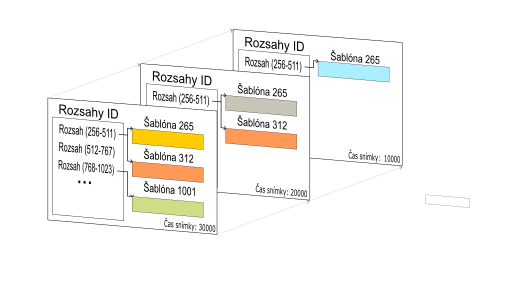
\includegraphics[width=0.8\textwidth]{kapitola_3/ipfixcol2_manager_snimky.pdf}
    \caption{Snímky manažéru v~priebehu procesu redefinície šablón}
    \label{ipfixcol2_snimky}
\end{figure}

\section{Zásuvné moduly}
\label{sec:ipfixcol2_moduly}

V~súčasnej dobe majú správcovia sietí využívajúci IPFIXcol2 na výber z~niekoľkých modulov, ktorých prehľad sa nachádza
v~tabuľke \ref{tab:ipfixcol2_moduly}. Konfigurácia modulov prebieha pomocou konfiguračného XML súboru, ktorý je spracovaný pri spustení kolektoru. Po načítaní nastavení jednotlivých modulov dochádza k~ich
inštanciácii jadrom a~kolektor začína spracovávať prichádzajúce IPFIX správy.

\vspace{1em}

\begin{table}[ht]
    \centering
    \aboverulesep=0ex
    \belowrulesep=0ex
    \renewcommand{\arraystretch}{1.2}
    \begin{tabular}{c|cp{8.6cm}}
         Typ modulu & Názov & Stručný popis\\ \toprule
         \multirow{2}{*}{Vstupný} & TCP, UDP & Komunikácia s~exportérom v~reálnom čase (online) \\
         & FDS, IPFIX & Načítavanie dát zo súborov (offline) \\ \midrule
         \multirow{3}{*}{Vnútorný} & anonymizačný & \multirow{3}{8cm}{Anonymizácia citlivých údajov, profilovanie a~filtrovanie tokov} \\
         & profilovací & \\
         & filtrovací & \\ \midrule
         \multirow{6}{*}{Výstupný} & FDS, IPFIX & Ukladanie informácií o~tokoch do súborov \\
         & json & Viacero možností exportu správ (server, súbor, text) \\
         & forwarder & Preposielanie správ ďalším kolektorom \\
         & viewer, timecheck & Textové zobrazenie správ, kontrola čas. razítok \\
         & lnfstore & Ukladanie do súborov vo formáte nástroja \textit{nfdump} \\
         & unirec & Export dát vo formáte nástroja \textit{Nemea} \\ \bottomrule
    \end{tabular}
    \caption{Moduly kolektoru IPFIXcol2}
    \label{tab:ipfixcol2_moduly}
\end{table} \newpage

Počas navrhovania kolektoru bol dôraz kladený na možnosť vytvárania nových modulov a~ich jednoduchú integráciu v~rámci kolektoru. Definícia nového modulu začína štruktúrou \texttt{ipx\_plugin\_info}, ktorá ho identifikuje spomedzi ostatných častí kolektoru. Každý modul musí
implementovať minimálne tri základné funkcie. Prvou z~nich je inicializačná funkcia (\texttt{ipx\_plugin\_init}). Jej úlohou je zabezpečiť vytvorenie privátnych dát (napr. databázového spojenia), s~ktorými modul pracuje v~priebehu svojej činnosti. Najdôležitejšou funkciou, ktorú
musí modul implementovať, je funkcia zabezpečujúca jeho hlavnú činnosť (\texttt{ipx\_plugin\_process}), ktorou je práca s~dátovými záznamami o~tokoch. V~rámci tejto funkcie sú realizované činnosti charakterizujúce daný modul. Poslednou povinnou funkciou je ukončenie činnosti
modulu (\texttt{ipx\_plugin\_destroy}) a~uvoľnenie všetkých zdrojov, ktoré ním boli alokované.

% -------------------------------------------  NÁVRH ------------------------------------------- %
% plánovaný rozsah: 30-40\% == cca 12-16 strán
% poznámky:
\chapter{Návrh obohacovania IPFIX správ}
\label{chpt:obohacovanie}

% \item spolu s~tým, ako sa vyvíjal kolektor od pôvodného IPFIXcol, tak sa dodatočne pracuje na "migrácií"  pôvodných častí do nového návrhu ... napr filtračný a profilovací modul v~práci od michala sedláka \cite{sedlak}
% \item obohacovanie správ konkrétne hodnotami ASN a GeoIP bola súčasťou pôvodnej architektúry kolektoru
Z~popisu práce kolektoru v~sekcii \ref{sec:collector_overview} vyplýva, že kolektor by mal okrem základnej činnosti spojenej s~ukladaním záznamov podporovať pokročilejšie operácie, ktorými sú napríklad filtrovanie, profilovanie, alebo obohacovanie tokov. Tieto funkcie, ktoré boli do istej miery
súčasťou pôvodného návrhu kolektoru IPFIXcol, však nebolo možné pri prechode na novú verziu aplikovať v~pôvodnej implementácii. Na základe tejto skutočnosti je nutné prispôsobiť ich novému návrhu, čomu sa venovala bakalárska práca Michala Sedláka \cite{sedlak} rozširujúca kolektor IPFIXcol2 o~možnosti
filtrovania a~profilovania tokov. Podobné ciele si kladie aj táto práca, ktorá je zameraná na obohacovanie tokov dátami z~externých zdrojov. Nový návrh obohacovania tokov je založený na rozšírení jadra kolektoru dvomi komponentmi. Prvým z~nich je modifikátor, ktorý realizuje
obohacovanie dátových záznamov a~taktiež zabezpečuje správu ich šablón. Druhým komponentom jadra je tvorca nových dátových správ s~modifikovanými záznamami, ktoré sú následne odosielané do zreťazenej linky.
Jednoduché vytváranie modulov následne ponúka možnosť rozšírenia nového kolektoru o~vnútorné moduly obohacujúce správy o~čísla autonómnych systémov (ASN) a~geografické informácie zdroja a~cieľa toku (GeoIP).

Táto kapitola sa zaoberá popisom nového návrhu obohacovania správ kolektoru IPFIX\-col2. V~jej úvode sú popísané autonómne systémy a~geolokácia spolu s~ich významom pri analýze dát.
Nasleduje stručné zhrnutie obohacovania správ pôvodnej verzie kolektoru obsahujúce zhodnotenie jeho pozitívnych a~negatívnych stránok, ktoré sú adresované v~novom návrhu.
Ďalej je jej súčasťou samotné obohacovanie záznamov kolektoru realizované pomocou nových komponentov jeho jadra. V~závere kapitoly sa nachádza stručná rekapitulácia činností nových vnútorných modulov realizujúcich úpravu záznamov
prechádzajúcich kolektorom.

% \item popis ASN, čo to je, na čo to je dobré
\section{Autonómne systémy a~geolokácia}
Pred zhodnotením návrhu obohacovania správ pôvodnej verzie kolektoru je nutné stanoviť si základné informácie, ktorými budú záznamy rozšírené. Na úvod je vhodné inšpirovať sa jedným z~modulov pôvodného kolektoru, ktorý obohacoval toky správ geolokačnými údajmi popisujúcimi zdroj a~cieľ
komunikácie. Ďalšou položkou obohacovania môžu byť čísla autonómnych systémov, pričom oba druhy týchto položiek predstavujú cenné informácie z~pohľadu analýzy prevádzky na sieti.

\textbf{Autonómne systémy} (AS) sú definované ako skupina IP sietí pod správou jedného operátora s~jasne definovanou smerovacou politikou \cite{rfc1930}. Typicky sa AS spája s~poskytovateľom internetových služieb (ISP) alebo inými organizáciami zabezpečujúcimi služby podobného charakteru. AS majú
využitie najmä pri smerovaní paketov putujúcich cez internet a~sú využívané smerovacími protokolmi, ktoré delíme na dve skupiny:

\vspace{-.5em}
\setlist[itemize]{itemsep=0mm}
\begin{itemize}
    \item \textbf{Interior gateway protocol} (IGP) -- skupina protokolov zabezpečujúca smerovanie v~rámci jedného AS (napr. OSPF, IS-IS, RIP)
    \item \textbf{Exterior gateway protocol} (EGP) -- protokol BGP zabezpečujúci smerovanie medzi viacerými AS
\end{itemize}

AS sú identifikované pomocou unikátnych čísel, ktoré sú spravované organizáciou IANA\footnote{Čísla registrovaných autonómnych systémov: \url{iana.org/assignments/as-numbers/as-numbers.xhtml}}. Analyzovanie informácií o~tokoch spojených s~autonómnymi systémami dáva správcom sietí lepší prehľad
o~prúdení toku dát cez sieť. Táto analýza sa môže následne využívať k~zlepšovaniu kvality služieb poskytovaných klientom, napríklad pri zisťovaní príčin výpadkov siete alebo kritických úsekov infraštruktúry.
Taktiež majú význam pri zvyšovaní bezpečnosti, keďže umožňujú odhadnutie potenciálne škodlivej komunikácie na základe reputačných databáz AS, ktoré určujú dôveryhodnosť komunikácie smerujúcej z~danej siete.

% \item popis GeoIP, čo to je, na čo to je dobré
Podobné využitie má \textbf{IP geolokácia}, ktorá určuje geografický zdroj a~cieľ toku na základe IP adries, ktoré sa v~ňom nachádzajú \cite{geoip}. Pri geolokácii sa môžu zisťovať rôzne atribúty pôvodu dát, pričom medzi najčastejšie
vyhľadávané patria: kód krajiny/regiónu, názov mesta alebo GPS súradnice. Výsledky získané touto metódou nemusia byť vždy spoľahlivé a~všeobecne platí, že pri zisťovaní polohy na úrovni súradníc sa presnosť výsledku znižuje.
V~takomto prípade súradnice nepopisujú presné miesto komunikujúceho zariadenia, ale iba jeho približnú polohu. Na základe tejto skutočnosti je v~praxi často preferovaná lokalizácia tokov na úrovni krajiny alebo mesta.
Výhodou geolokácie je možnosť zvýšenia bezpečnosti vo forme obmedzenia prístupu ku sieti pre zariadenia na základe ich polohy. Taktiež môžu organizácie využívajúce GeoIP zlepšovať kvalitu poskytovaných služieb, kedy v~závislosti od
počtu užívateľov pripojených z~rovnakej oblasti môže napríklad dôjsť ku zavedeniu podporných lokálnych serverov poskytujúcich danú službu pre túto oblasť.

\section{Zhodnotenie pôvodného návrhu}
\label{sec:zhodnotenie_navrhu}
Pôvodný návrh kolektoru IPFIXcol sa čiastočne venoval aj problematike obohacovania tokov o~dáta z~externých zdrojov. Príkladom je GeoIP modul, ktorý pridával do dátových záznamov číselné kódy\footnote{Trojciferné čísla identifikujúce
krajinu podľa štandardu ISO 3166-1} krajín na základe zdrojovej a~cieľovej IP adresy toku. Úskalia pôvodného návrhu súvisia so spôsobom, akým kolektor pracoval s~prijatými IPFIX správami. Podobne ako pri novom kolektore sa aj v~pôvodnej verzii
využívajú dátové správy, ktorých dôležitým prvkom pre obohacovanie tokov je dodatočná štruktúra \textbf{metadát}.

% \begin{figure}[ht]
%     \centering
%     \includegraphics[width=0.5\textwidth]{kapitola_4/ipfixcol_datova_sprava.pdf}
%     \caption{Štruktúra metadát dátovej správy kolektoru IPFIXcol}
%     \label{fig:ipfixcol_datova_sprava}
% \end{figure}

V~dátovej správe je každý záznam spojený s~metadátami obsahujúcimi informácie spojené s~autonómnymi systémami, geografickými údajmi alebo profilmi charakterizujúcimi daný záznam. Pre uvedenie príkladu práce s~touto štruktúrou sa môžeme pozrieť na činnosť GeoIP modulu na obrázku
\ref{fig:stare_obohacovanie}. Jeho práca začína iteráciou cez záznamy dátovej správy. Pre každý záznam je nájdená zdrojová a~cieľová IP adresa, ktoré sú následne použité pri vyhľadaní geolokačných informácií v~databáze. Výsledok vyhľadávania (textový reťazec označenia krajiny, napr. CZ, SK, UK) je
neskôr použitý pri vyhľadaní číselného kódu v~tabuľke kódov krajín. Tento kód je vložený do štruktúry metadát pre práve obohacovaný záznam. Nevýhodou tohto prístupu je skutočnosť, že tabuľka kódov krajín je priamou súčasťou zdrojového kódu modulu, čo sťažuje jej prípadnú aktualizáciu.

\begin{figure}[ht]
    \centering
    \includegraphics[width=0.8\textwidth]{kapitola_4/ipfixcol_obohacovanie.pdf}
    \caption{Obohacovanie správ modulom GeoIP v~kolektore IPFIXcol}
    \label{fig:stare_obohacovanie}
\end{figure}

Pri implementácii obohacovania správ nového kolektoru možno využiť rovnaký návrh rozšírenia dátovej správy o~štruktúru metadát. Tento prístup má viacero nevýhod, pričom najhlavnejšou z~nich je nízka flexibilita pridaných informácií.
Ďalšou z~nevýhod je fakt, že pridané informácie nie sú súčasťou surovej správy, a~teda moduly kolektoru musia s~týmito dátami pracovať separátne. Z~daných skutočností vyplýva nepriaznivý dôsledok spočívajúci v~úprave implementácie
ostatných častí kolektoru pracujúcich s~touto štruktúrou pri pridaní nových obohacujúcich položiek. Navyše, ak by kolektor neobsahoval aktívny ASN alebo GeoIP modul, štruktúra metadát by ostala nevyplnená,
čo by museli vedieť rozpoznať výstupné moduly. Z~tohto dôvodu by musel kolektor obsahovať mechanizmus označujúci platné a~neplatné položky štruktúry metadát, čo by spôsobovalo zbytočné komplikácie pri pridávaní nových položiek tokov.
Obohacovanie tokov hodnotami čísel AS je navyše v~predošlej verzii kolektoru úplne vynechané.

\section{Nový návrh obohacovania správ}
\label{sec:novy_navrh_obohacovania}

Na základe negatívnych aspektov starého návrhu je potrebné vyvinúť nový spôsob, ktorým bude kolektor IPFIXcol2 schopný toky obohacovať. Základnou myšlienkou nového návrhu je pridávanie obohacujúcich dát priamo do surovej správy. Tento spôsob zahŕňa úpravu záznamov dátových správ, ale taktiež
šablón popisujúcich tieto záznamy. Medzi výhody tohto návrhu patrí zvýšená flexibilita, ktorá umožňuje obohacovanie tokov o~ľubovoľné informácie bez nutnosti úpravy ostatných častí kolektoru. Jednu z~nevýhod tohto návrhu však predstavuje značná komplikovanosť úkonov spojených s~udržiavaním
modifikovaných šablón, čo môže mať negatívny dopad na výkonnosť kolektoru. Z~toho dôvodu sú súčasťou kapitoly \ref{chpt:implementacia} testy hodnotiace dopady obohacovania správ na výkonnosť kolektoru.

\begin{figure}[ht]
    \centering
    \includegraphics[width=0.8\textwidth]{kapitola_4/ipfixcol2_obohacovanie.pdf}
    \caption{Nový návrh obohacovania správ v~kolektore IPFIXcol2}
    \label{fig:nove_obohacovanie}
\end{figure}

Postup obohacovania správ zobrazený na obrázku \ref{fig:nove_obohacovanie} je založený na dvoch nových komponentoch jadra kolektoru. Prvým z~nich je \textbf{modifikátor záznamov}, ktorý poskytuje obohacujúcemu modulu funkcie na úpravu
dátových záznamov a~šablón. Výsledkom činnosti modifikátoru sú obohatené záznamy, ktoré sú uložené v~dátovej správe vytvorenej \textbf{tvorcom nových správ}. Celú činnosť obohacovania zastrešuje vnútorný \textbf{obohacujúci modul}, ktorý
prepája tieto novovytvorené komponenty a~poskytuje informácie potrebné k~obohateniu záznamov. Následne sú upravené správy odosielané namiesto pôvodných neobohatených do zreťazenej linky, cez ktorú putujú až do výstupných modulov kolektoru.

\subsection*{Modifikácia dátových záznamov}
Vnútorné moduly upravujúce dátové záznamy nad nimi typicky realizujú dve činnosti. Prvou z~nich je pridávanie nových položiek, pri ktorom musí vnútorný modul tieto položky definovať a~zároveň poskytnúť modifikátoru funkciu na získavanie
ich hodnôt. Nové položky sú následne pridané do každého dátového záznamu prechádzajúcim vnútorným modulom. Druhou činnosťou je filtrovanie vybraných položiek vyskytujúcich sa v~prijatých tokoch, ktoré má za následok ich odobratie zo záznamu.
Pri tejto činnosti musí vnútorný modul predať modifikátoru informáciu o~pozícií týchto položiek určených na filtrovanie. Modifikátor následne zastrešuje prácu spojenú so samotným obohacovaním a~filtrovaním položiek tokov.

Nový komponent modifikátoru pracuje na úrovni jednotlivých dátových záznamov získaných z~prijatých správ. Základom jeho činnosti je definovanie obohacovacej a~filtrovacej funkcie, ktoré sú využívané v~priebehu jeho činnosti ako tzv. \textit{callback}
funkcie. Tieto funkcie sú implementované vnútornými modulmi využívajúcimi modifikátor k~úprave dátových záznamov. Obohacovacia funkcia slúži k~získavaniu hodnôt nových položiek pre každý spracovávaný záznam toku.
Okrem nej však musí vnútorný modul poskytnúť modifikátoru taktiež definície nových položiek, ktoré majú byť do záznamu pridané. Ich formát je totožný s~definíciou položky šablóny štandardu IPFIX 7011
(obrázok \ref{ipfix_sablona}). V~prípade filtrovania je proces modifikácie jednoduchší a~realizuje sa pomocou filtrovacej funkcie, ktorá v~rámci šablóny definuje pozície položiek určených na odstránenie.

Na obrázku \ref{fig:modifier_example} je zobrazený ilustračný príklad obohatenia zjednodušeného dátového záznamu položkami \texttt{InterfaceName} a~\texttt{packetTotalCount}. Prvým krokom v~procese obohacovania záznamu je rozšírenie šablóny
novými položkami realizované modifikátorom po prijatí dátového záznamu. Následne je na základe obohacovacej funkcie naplnená vnútorná štruktúra modifikátoru obsahujúca získané hodnoty nových položiek.
Pre každú novú položku je okrem hodnoty získaná aj jej veľkosť, ktorá zároveň určuje jej použitie v~upravenom toku nasledovným spôsobom: \newpage

\setlist[enumerate]{itemsep=0mm}
\begin{enumerate}
    \item veľkosť položky $\geq$ 0: hodnota položky je platná a~použije sa pri obohatení toku
    \item veľkosť položky $<$ 0: hodnota položky je neplatná (napr. v~prípade, že ju z~dôvodu absencie záznamu v~databáze nebolo možné určiť) a~použije sa typická hodnota reprezentujúca prázdnu položku
        (v~prípade číselného typu položky hodnota nula, v~prípade položiek s~variabilnou dĺžkou prázdne pole)
    \item veľkosť položky $=$ rezervovaná hodnota: položka nie je súčasťou upraveného záznamu (napr. z~dôvodu existencie danej položky v~aktuálne obohatenom toku)
\end{enumerate}

Hodnoty nových položiek sú modifikátorom následne vložené z~vnútornej štruktúry do nového dátového záznamu.

\begin{figure}[ht]
    \centering
    \includegraphics[width=\textwidth]{kapitola_4/modifier_example.pdf}
    \caption{Príklad obohatenia dátového záznamu}
    \label{fig:modifier_example}
\end{figure}

% šablóny sú uchovávané v~manažéri šablón, pričom je pre každý aktuálne otvorené transportné sedenie + ODID vytvorený separátny manažér, ktorý je uložený v~kontexte modifikátoru
% ku vytvoreniu nového kontextu dochádza pri tom, ak modifikátor narazí na správu z~sedenia+ODID, ktoré ešte nevidel ... navyše musí byť schopný reagovať aj na ukončovanie sedení v~podobe správ sedení
% modifikátor musí riešiť aj vytváranie nových čísel šablón -> v~kontexte sa okrem manažéru nachádza aj číslo posledne použitej šablóny, ktoré sa postupne inkrementuje ... môžu sa tieto čísla opakovať v~rámci
%   sedení? => áno, pretože kontext šablóny je platný v~rámci ODID + sedenia .. čo sa stane, ak mu dojdú čísla? => reštartuje kontext pre danú doménu a pomodlí sa, aby ich prišlo menej
Typicky je v~kolektore IPFIXcol2 za správu šablón zodpovedný preprocesor, ktorý spracováva prijaté IPFIX správy. Je potrebné zdôrazniť, že so zmenou šablón popisujúcich dátové záznamy sa zodpovednosť ich správy presúva na modifikátor.
Šablóny sú v~modifikátore po ich úprave uložené v~manažéri šablón príslušného \textbf{kontextu sedenia}. Potreba prepojenia šablóny na kontext sedenia vyplýva zo skutočnosti, že v~rámci jednotlivých spojení môžu byť odlišné šablóny
identifikované rovnakým číslom. Kontext sedenia, ktorý je zobrazený na obrázku \ref{fig:modifier_ctx}, slúži na správu upravených šablón odosielaných z~rovnakej pozorovacej domény. Kľúčovou položkou kontextu sedenia je dvojica
identifikátoru transportného sedenia s~exportérom a~ODID, ktorá jednoznačne identifikuje zdroj pôvodnej šablóny. Na prvý pohľad sa môže zdať, že ku vytvoreniu kontextu sedenia dochádza bezprostredne po ustanovení nového spojenia s~exportérom.
Tento proces je však zrealizovaný až po prijatí prvej správy z~novej pozorovacej domény daného exportéru.

Kontext sedenia obsahuje okrem manažéra šablón aj ID nasledujúcej šablóny, ktoré sa používa pri generovaní sekvencie nových identifikačných čísel upravených šablón.
Príčinou generovania nových identifikátorov šablón je skutočnosť, že záznamy popísané jednou šablónou sa môžu po obohatení namapovať na viacero odlišných záznamov v~závislosti od toho, či sa pôvodný záznam podarilo obohatiť modulom
o~nové dáta, alebo či sa modifikátor rozhodol tieto položky ignorovať. Pri filtrovaní môže taktiež nastať podobná situácia, v~prípade, že sa viacero pôvodných záznamov namapuje na rovnaký záznam, ak sú niektoré položky zo šablóny odobrané.
V~zriedkavých situáciách môže byť počet nových šablón väčší ako je maximálna hodnota počítadla identifikátorov (65535). V~takom prípade dochádza ku reštartovaniu kontextu sedenia, ktoré zahŕňa odstránenie všetkých
definovaných šablón v~manažéri spolu s~nastavením ID nasledujúcej šablóny na predvolenú hodnotu (256). Obohacovanie tokov následne môže bezproblémovo pokračovať ďalej.

\begin{figure}[ht]
    \centering
    \includegraphics[width=0.6\textwidth]{kapitola_4/modifier_ctx.pdf}
    \caption{Štruktúra kontextu sedenia modifikátoru tokov}
    \label{fig:modifier_ctx}
\end{figure}

% na čo je mapovanie šablón, ukázať štruktúru
% mapovanie šablón je na to, aby sa nemuseli prechádzať všetky snapshoty a zisťovať, či niekde je už takáto šablóna ... čo by v prípade veľkého počtu šablón bolo pomalé
% podobne ako v preprocesore sa to využíva fakt, že počet šablón je konečný a preto je možné vytvoriť 2 úrovňovú adresovaciu tabuľku
Pred uložením modifikovanej šablóny do manažéra šablón je z~dôvodu eliminácie duplikátneho ukladania dôležité skontrolovať, či sa konkrétna šablóna v~manažéri už nevyskytuje. Riešenie, ktorým disponuje manažér šablón, je porovnávanie
novej šablóny so šablónami uloženými v~rámci aktuálnej snímky. V~prípade veľkého počtu vygenerovaných šablón však môže sekvenčné prechádzanie snímky zvýšiť čas potrebný k~nájdeniu modifikovanej šablóny, čo môže mať negatívny dopad na
výkonnosť kolektoru. Kontext sedenia preto obsahuje štruktúru \textbf{mapovania upravených šablón} urýchľujúcu ich vyhľadávanie. Štruktúra mapy modifikovaných šablón, podobná snímke manažéra šablón (obrázok \ref{ipfixcol2_snimky}), je
tvorená dvojúrovňovou adresovacou tabuľkou, pričom prvá vrstva rozdeľuje rozsah identifikátorov šablón na rovnako veľké intervaly. Druhá vrstva je indexovaná identifikačným číslom pôvodnej šablóny a~obsahuje lineárne viazaný zoznam
s~definíciami modifikovaných šablón, ktoré vznikli zo šablóny s~daným identifikátorom (obrázok \ref{fig:modifier_mapper}). Dĺžka tohoto zoznamu sa odvíja od toho, na aký počet šablón sa môže potenciálne po obohatení namapovať pôvodná šablóna.
Vo väčšine prípadov sa dĺžka zoznamu pohybuje rádovo v~jednotkách položiek, čo významne napomáha zvyšovaniu rýchlosti procesu vyhľadávania modifikovanej šablóny.

Pri procese správy upravených šablón (ich uloženie v~manažéri) sa komponent modifikátoru pokúsi o~nájdenie rovnako definovanej šablóny v~mape modifikovaných šablón. V~prípade úspechu tak nemusí byť šablóna pracne vyhľadávaná v~manažéri a~modifikátor môže
pracovať s~odkazom získaným z~položky mapy. V~opačnom prípade je nutný sekvenčný prechod aktuálnej snímky z~dôvodu možnej existencie rovnako upravenej šablóny vytvorenej zo šablóny s~odlišným identifikačným číslom. V~prípade, že na
takúto šablónu modifikátor narazí, vytvorí v~mape modifikovaných šablón na indexe pôvodnej šablóny novú položku, ktorá bude obsahovať odkaz na upravenú šablónu. Tento proces zaisťuje, že modifikovaná šablóna je následne uložená v~manažéri šablón
príslušného kontextu sedenia a~môže byť použitá na popis obohateného záznamu. Na konci procesu obohatenia je upravený dátový záznam vrátený vnútornému modulu využívajúcemu modifikátor (ASN, GeoIP, \ldots).

\begin{figure}[ht]
    \centering
    \includegraphics[width=\textwidth]{kapitola_4/mapper.pdf}
    \caption{Mapovanie pôvodných šablón na modifikované}
    \label{fig:modifier_mapper}
\end{figure}

% podobne ako preprocesor sa tu využívajú odpadové správy na odosielanie nepoužívaných šablón
Súčasťou správy šablón je aj reakcia na ukončenie spojenia s~exportérom, pri ktorej dochádza k~odstráneniu šablón definovaných daným exportérom z~dôvodu nutnosti uvoľnenia pamäte potrebnej pre ich uloženie. V~modifikátore dochádza po prijatí správy sedenia s~príznakom ukončenia spojenia
k~odstráneniu príslušnej položky kontextu sedenia, ktorá je spätá s~daným spojením. Zároveň sú všetky nové šablóny tohoto kontextu vložené do odpadovej správy a~následne odoslané do zreťazenej linky. Je dôležité podotknúť, že odstránenie položky kontextu nie je spojené s~ODID, ale výhradne
s~identifikátorom transportného sedenia. Po ukončení spojenia s~exportérom tak dochádza k~odstráneniu všetkých s~ním súvisiacich kontextov (nezávisle od ODID).

% Manažér šablón odstraňuje v~priebehu svojej činnosti definície šablón, ktoré sa v~priebehu činnosti kolektoru stali neplatnými (napr. po vypršaní časového limitu protokolu UDP). Keďže mapovanie modifikovaných šablón obsahuje ich odkazy,
% je po odstránení neplatných šablón nutné vymazať z~manažéra všetky položky s~prípadnými neplatnými odkazmi na upravené šablóny. Z~toho dôvodu je v modifikátore zavedený limit počtu položiek mapovania. Po prekročení tohto limitu dochádza
% k odstráneniu všetkých položiek mapovania a eliminácii neplatných šablón z manažéra.

\subsection*{Vytváranie nových dátových správ}

Po ukončení procesu modifikácie je nutné uložiť dátové záznamy do novovzniknutých dátových správ. Táto činnosť je realizovaná tvorcom dátových správ, ktorý je novým komponentom jadra kolektoru. Proces tvorby dátovej správy je založený
na vytvorení surovej IPFIX správy s~upravenými dátovými záznamami, nad ktorými následne vzniká obálka dátovej správy, ktorá je ďalej odoslaná do zreťazenej linky kolektoru.

% vytváranie novej správy začína predaním hlavičky pôvodnej správy, ktorá je prekopírovaná do novej správy (čo znamená že má rovnaké ODID, sekvenčné číslo, atď)
% hlavnou funkciou je pridávanie dátových záznamov, keďže dátové záznamy musia byť v~sade, ktorá obsahuje ID definujúcej šablóny, tak je vytváranie sád zabezpečené automaticky
V~priebehu procesu vytvárania novej surovej IPFIX správy dochádza k~okopírovaniu hlavičky pôvodnej správy z~dôvodu potreby zachovania sekvenčného čísla, času exportu a~ODID, ktoré sú súčasťou pôvodnej správy. Tvorca nových správ ďalej poskytuje
zastrešujúcemu modulu, t.j. vnútornému modulu implementujúcemu logiku obohacovania alebo filtrovania tokov (napr. ASN alebo GeoIP), funkcie na pridávanie modifikovaných dátových záznamov. V~priebehu procesu pridávania záznamu je automaticky vytvorená nová dátová sada
s~identifikačným číslom šablóny záznamu. V~prípade záznamov špecifikovaných rovnakou šablónou dochádza k~ich uloženiu v~rámci rovnakej dátovej sady, ako je ukázané na obrázku \ref{fig:builder}.

\begin{figure}[ht]
    \centering
    \includegraphics[width=0.5\textwidth]{kapitola_4/builder.pdf}
    \caption{Pridávanie dátových záznamov do novej surovej IPFIX správy}
    \label{fig:builder}
\end{figure}

% je možné si všimnúť, že takto vytvorené správy neobsahujú v~sebe definície šablón ... je to problém? nie, pretože sa v~kolektore so surovými šablónami nepracuje priamo, ale cez vnútorné štruktúry kolektoru.
%   A~čo ak chce kolektor odosielať IPFIX správy so šablónami inému kolektoru? To rieši výstupný modul tým, že pracuje ako exportér a separátne odosiela definície šablón opäť definované vo vnútornej štruktúre ...
% poslednou časťou je ukončenie správy, ktoré zabezpečí vytvorenie novej dátovej správy (teda obálku s~odkazmi na sady/záznamy), ktorá sa ďalej môže posielať do kolektoru
Samotné šablóny nie sú po pridaní dátového záznamu súčasťou novovytvorených správ, čím dochádza ku redukcii veľkosti surovej správy. Zároveň sa tu však vyskytuje otázka, či absencia šablón v~správach nemá vplyv na fungovanie ostatných častí kolektoru. Pri práci ostatných častí
kolektoru s~dátovými záznamy sa využívajú výhradne spracované šablóny, ktoré sú odkazované zo záznamov v~obálke dátovej správy. Moduly a~časti jadra kolektoru (s~výnimkou preprocesoru) tak nepristupujú priamo k~šablónam surovej správy. Špeciálnym prípadom, na ktorý je dôležité upozorniť, je výstupný
\textit{forwarder} modul, ktorý sa používa na distribúciu prijatých správ na subkolektory. Pokiaľ by odosielal výlučne surové IPFIX správy, ich interpretácia by z~dôvodu absencie šablón nebola možná. \textit{Forwarder} modul však odošle definície šablón uložené v~snímkach manažéra šablón skôr,
než samotné správy, preto ani v~tomto prípade nie je pridávanie šablón do surových správ potrebné. Po vložení všetkých záznamov je nad novou surovou IPFIX správou vytvorená obálka dátovej správy, ktorá je následne vrátená zastrešujúcemu modulu.

\section{Popis činnosti zastrešujúcich modulov}

% moduly následne využívajú modifikátor a komponent tvorby správ
% pre modifikátor poskytujú funkcie na získavanie dát (ktorá často pracuje s nejakou databázou) a filtru
Poslednou časťou nového návrhu sú zastrešujúce moduly (vnútorné moduly kolektoru realizujúce obohacovanie alebo filtrovanie tokov), ktoré spájajú činnosti nových komponentov jadra kolektoru. Pri ich inštanciácii sú inicializované komponenty
modifikátoru a~tvorcu správ, ktoré sú využívané v~priebehu ich práce. Pred vytvorením modifikátoru je nutné definovať príslušné callback funkcie, ktoré budú použité v~priebehu úpravy záznamov. Tieto funkcie implementujú logiku
úpravy záznamov, t.j. pri obohacovaní určujú spôsob získania hodnôt nových položiek a~pri filtrovaní určujú pozície položiek určených k~odstráneniu.

% musí sa prihlásiť na odber správ sedenia, aby mohol modifikátoru oznamovať ukončenie spojenia s exportérom a odstránenie nim definovaných šablón
Pri inicializácii zastrešujúceho modulu je potrebné jeho prihlásenie na odber správ sedenia. Po prijatí správy sedenia oznamujúcej ukončenie spojenia s~exportérom, je táto informácia predaná modifikátoru záznamov, ktorý môže následne uvoľniť šablóny definované v~tomto spojení.

% následne postupne prechádza záznamy dátovej správy
% zavolá nad záznamom funkciu modifikátoru aby ich upravili
% upravený záznam vloží do novej správy
Po prijatí novej dátovej správy je jej kontext odoslaný do modifikátoru, ktorý na jeho základe aktualizuje kontext sedenia pre danú správu. Zároveň je tvorcom správ vytvorená nová surová IPFIX správa obsahujúca hlavičku pôvodnej správy. Zastrešujúci modul ďalej prechádza všetkými dátovými záznamami
prijatej správy, ktoré sú odoslané modifikátoru k~úprave. Upravené dátové záznamy sa vkladajú do novej správy v~tvorcovi správ.

% po spracovaní všetkých záznamov je správa odoslaná do zreťazenej linky
Po úspešnom spracovaní všetkých záznamov pôvodnej správy je vytvorená nová dátová správa, ktorá je odoslaná do zreťazenej linky kolektoru. Pokiaľ dôjde ku chybe v~niektorej z~časti jadra kolektoru, je namiesto novej správy odoslaná pôvodná, preto následne nevzniká riziko prípadnej straty
dát pri výskyte chyby v~obohacovaní.

% ------------------------------------  IMPLEMENTÁCIA A TESTOVANIE ------------------------------------ %
% plánovaný rozsah: 20-30\% == cca 8-12 strán
% poznámky: väčšina vecí bude popísaná v predchadzajúcej kapitole, tu sa skôr sústrediť na rozdelenie do komponent

\chapter{Realizácia obohacovania správ a~testovanie}
\label{chpt:implementacia}

Predposledná kapitola popisuje implementáciu nových komponentov jadra kolektoru a~obohacujúcich modulov. Taktiež sú v~nej zhodnotené výsledky výkonnostných testov merajúcich priepustnosť kolektoru pri použití nového návrhu obohacovania záznamov.

% \item implementácia v~jazyku C, CMake na preklad, Doxygen na komentáre, google tests na jednotkové testy
Implementácia nových častí kolektoru je napísaná v~jazyku C a~na kompiláciu kolektoru sa využíva prekladový systém \textit{CMake}\footnote{\url{https://cmake.org/}}. Preklad kolektoru, spolu s~knižnicou \textit{libfds}, potrebnou na jeho činnosť, je popísaný v~prílohe \ref{appendix:source}.
Dokumentácia nových častí kódu je vytvorená, rovnako ako vo zvyšných častiach kolektoru, pomocou nástroja \textit{Doxygen}\footnote{\url{https://www.doxygen.nl/}}. V~rámci testovania boli pre nové komponenty jadra vytvorené jednotkové testy, ktoré sa zameriavali na úpravu
záznamov, nastavenie kontextu modifikátoru a~vytváranie nových správ. Tieto testy boli realizované pomocou knižnice \textit{Google Tests}\footnote{\url{https://github.com/google/googletest}}.

% popis testovacieho stroja .. že mi v rámci spolupráce s týmom liberouter bol poskytnutý servar "sevar" na ktorom prebiehali testy
% ako testy fungujú?
%   záznamy sú na kolektor odosielané pomocou nástroja \textit{ipfixsend2}, ktorý slúži na testovanie kolektoru a umožňuje
%   základom je konfiguračný súbor, ktorý obsahuje jeden TCP modul, ktorý prijíma dáta, zároveň je po ustanovení spojenia s exportérom zaznamenaný čas spustenia testovania
%   posledným modulom je ukážkový (dummy) modul, ktorý vypisuje štatistiky počtu spracovaných záznamov a po jeho ukončení je ukončené meranie času
Testovanie výkonnosti prebiehalo na fyzickom stroji, ku ktorému mi bol poskytnutý prístup v~rámci spolupráce s~tímom Liberouter organizácie CESNET. Parametre tohoto zariadenia a~prekladu je možné vidieť v~tabuľke \ref{tab:testovaci_stroj}. Na stroji počas výkonnostného testovania neprebiehali žiadne iné výpočetne
náročné úlohy. Samotné testovanie bolo založené na spustení kolektoru s~jedným vstupným TCP modulom. Testovacie dáta boli na kolektor odosielané prostredníctvom nástroja \textit{ipfixsend2}, ktorý je súčasťou kolektoru a~slúži k~jeho testovaniu. Ako výstupný modul bol použitý ukážkový
(\textit{dummy}) modul, ktorý zobrazuje štatistiky o~spracovaných správach po ukončení činnosti kolektoru. Okrem týchto modulov sa v~konfigurácii nachádza testovaný vnútorný modul, ktorý realizuje obohacovanie tokov. Cieľom testov je zistenie výkonnosti kolektoru, ktorá je vypočítaná ako podiel
celkového počtu záznamov a~času od prijatia dát vstupným TCP modulom až po ukončenie práce výstupného modulu.

Sady IPFIX záznamov zachytených z~pozorovania tokov na sieti, ktoré boli použité pri výkonnostných testoch, mi boli poskytnuté Ing. Lukášom Hutákom. Prvá z~nich, v~testoch označovaná ako \textit{bežná}, obsahuje IPFIX záznamy so základnými meranými vlastnosťami tokov. Druhá sada,
v~testoch tiež označovaná ako \textit{aplikačná}, obsahuje navyše položky získané z~aplikačných vrstiev (napr. DNS alebo HTTP). Výkonnosť kolektoru je taktiež podmienená typom položiek vyskytujúcich sa v~prijatých správach. Je teda dobré podotknúť, že správy v~bežnej sade obsahujú výhradne položky
so statickou dĺžkou, zatiaľ čo v~záznamoch aplikačnej sady sa vyskytujú tiež položky s~variabilnou dĺžkou. V~rámci týchto sád sú navyše generované IPFIX správy s~postupne narastajúcimi veľkosťami, čo umožňuje zistenie priepustnosti kolektoru v~závislosti od počtu záznamov vyskytujúcich sa v~prijatých
správach.

\begin{table}[ht]
    \centering
    \begin{tabular}{cc}
        \toprule
        Procesor & Xeon (R) CPU E5-2630 v3 @ 2.40GHz \\
        Počet jadier & 8 \\
        RAM & 64GiB \\
        Operačný systém & Scientific Linux \\
        Verzia OS & release 7.9 (Nitrogen) Kernel 3.10.0-1160.25.1.el7.x86\_64 \\
        Použité nástroje & gcc 4.8.5, cmake 2.8.12.2 \\
        Typ prekladu & optimalizácia O2, bez ladiacich symbolov \\
        \bottomrule
    \end{tabular}
    \caption{Informácie o~použitom testovacom prostredí}
    \label{tab:testovaci_stroj}
\end{table}

K~porovnaniu výkonnosti nových častí kolektoru bola zvolená konfigurácia kolektoru obsahujúca vnútorný anonymizačný modul. Pri týchto testoch bol zvolený jednoduchý anonymizačný algoritmus, v~rámci ktorého je zachovaná vrchná polovica IP adresy a~jej zvyšok je vynulovaný. Výber tejto konfigurácie nám
poskytuje základnú predstavu o~priepustnosti kolektoru pri použití modulu pracujúceho priamo s~dátovými záznamami prijatých správ. Výsledky testu výkonnosti kolektoru s~anonymizačným modulom je možné vidieť v~grafe \ref{fig:tests_anon}.

\begin{figure}[ht]
    \centering
    \includegraphics[width=\textwidth]{kapitola_5/anon.pdf}
    \caption{Výkonnosť kolektoru s~anonymizačným modulom}
    \label{fig:tests_anon}
\end{figure}

Horná hranica priepustnosti kolektoru pri anonymizácii tokov je približne 8 miliónov záznamov za sekundu, pričom pri aplikačnej sade je to o~2 milióny záznamov menej. Tento pokles výkonnosti je spôsobený výskytom položiek premenlivej veľkosti v~aplikačnej sade.
Zároveň si môžeme všimnúť, že výkonnosť sa zvyšuje s~narastajúcou veľkosťou prijatých IPFIX správ.
Táto skutočnosť je zapríčinená zvyšujúcim sa počtom dátových záznamov vo väčších správach, čím dochádza ku zníženiu nákladov spojených s~réžiou práce so samotnými správami.

\section{Ukážkový obohacujúci modul}

% na testovanie bol vytvorený jednoduchý ukážkový obohacujúci modul, ktorý je konfigurovateľný pomocou XML ako ostatné časti ...
Za účelom testovania bol vytvorený ukážkový modul obhacujúci toky na základe zvolenej konfigurácie, ktorú je možné vidieť v~prílohe \ref{appendix:configuration}.
Konfigurácia tohto modulu obsahuje definície nových položiek, ktorými môže byť celé/desatinné číslo alebo textový reťazec. Zároveň sa v~konfigurácii nachádzajú hodnoty nových položiek, ktoré sú použité pri samotnom obohacovaní tokov.
Táto skutočnosť umožňuje izolovane otestovať výkonnosť nových častí jadra kolektoru bez nutnosti vyhľadávania hodnôt nových položiek v~databáze alebo inom zdroji dát. Toto vyhľadávanie sa v~ďalších testoch preukáže ako časovo kritický úsek procesu
obohacovania. Graf \ref{fig:tests_dummy_noopt} zobrazuje výkonnosť kolektoru s~ukážkovým obohacujúcim modulom po pridaní dvoch celočíselných položiek.

\begin{figure}[ht]
    \centering
    \includegraphics[width=\textwidth]{kapitola_5/dummy_noopt.pdf}
    \caption{Výkonnosť kolektoru s~ukážkovým obohacujúcim modulom}
    \label{fig:tests_dummy_noopt}
\end{figure}

Výsledky testovania ukážkového modulu zobrazujú zníženie priepustnosti kolektoru pri bežnej dátovej sade v~porovnaní s~anonymizačným modulom na hranicu 1,5 milióna záznamov za sekundu. Tento výrazný pokles je zapríčinený skutočnosťou, že oproti anonymizačnému modulu vykonáva
obohacujúci modul pokročilejšie operácie v~podobe zmeny štruktúry záznamov a~ich šablón pre každý prijatý dátový záznam.

\section{Moduly ASN a~GeoIP}

% používanie databáz od MaxMindDB (nejaký odkaz na to) a ich API na prácu s~nimi
Dôležitou súčasťou práce modulov ASN a~GeoIP, ktorá v~tejto práci doposiaľ nebola popísaná, je získavanie geolokačných informácií a~čísel autonómnych systémov. V~súčasnosti sú v~rámci implementácie spomínaných modulov na túto aktivitu využívané voľne dostupné databázy
\textit{GeoLite2}\footnote{K ich stiahnutiu je potrené vytvorenie účtu. Pri testovaní boli využité nespoplatnené databázy dostupné na: \url{https://dev.maxmind.com/geoip/geolite2-free-geolocation-data}} vyvíjané organizáciou MaxMind. Pri ich výbere je možné siahnuť po dvoch variantách --
textový formát CSV alebo interný formát MMDB (\textit{Max\-Mind Da\-ta\-Base}). Z~hľadiska výkonnosti boli v~implementácii využité databázy interného formátu, ktoré predstavujú v~porovnaní s~textovým formátom optimalizovaný spôsob vyhľadávania potrebných informácií.
Záznamy tohoto typu sú uložené v~štruktúre binárneho stromu, pričom je optimalizovaný aj samotný proces vyhľadávania, ktorý je popísaný spolu s~formátom MMDB vo verejnej dokumentácii\footnote{Popis formátu MMDB: \url{https://maxmind.github.io/MaxMind-DB/}}. Pri implementácii bola
k~práci s~týmito databázami využitá knižnica \textit{libmaxminddb}\footnote{GitHub stránky knižnice: \url{https://github.com/maxmind/libmaxminddb}}.

Vytvorenie odkazu na databázový objekt prebieha v~inicializačnej funkcii obohacovacieho modulu. Tento odkaz je následne predaný do modifikátoru prostredníctvom dát, ktoré sú využité pri volaní obohacovacej (callback) funkcie. Modifikátor v~priebehu obohacovania toku túto funkciu invokuje a~predá
jej odkaz na tieto dáta. Počas jej činnosti dochádza ku vyhľadaniu potrebných informácií z~uloženého databázového odkazu pomocou IP adresy získanej z~aktuálne spracovávaného záznamu toku. Pokiaľ záznam už položky určené na obohatenie obsahuje, ich pridanie do záznamu je vynechané.
Získané dáta sú obohacovacou funkciou vložené do vnútornej štruktúry modifikátoru, ktorý následne pokračuje v~činnosti úpravy dátového záznamu. V~priebehu ukončenia činnosti modulu je odkaz na databázu bezpečne odstránený.

% popis konfigurácie (možno v~prílohe), že ASN pridáva defaultne položky bgpSourceNumber a bgpDestinationNumber pre šablóny, ktoré tieto položky už neobsahujú
Modul ASN využíva na vyhľadávanie čísel AS binárnu databázu \textit{GeoLite2-ASN}. Pri konfigurácii tohto modulu je potrebné vopred definovať cestu ku tejto databáze, vďaka ktorej je následne prípadná aktualizácia jednoduchšia.
Čísla autonómnych systémov definované informačnými elemetami \texttt{bgpSourceAsNumber} a~\texttt{bgpDestinationAsNumber}, ktorými sú toky obohacované, sa nachádzajú v~spoločnom rozsahu informačných elementov organizácie IANA.

\vspace{-1em}
\begin{figure}[ht]
    \centering
    \includegraphics[width=\textwidth]{kapitola_5/asn_noopt.pdf}
    \caption{Výkonnosť kolektoru pri použití modulu ASN}
    \label{fig:tests_asn_noopt}
\end{figure}

% možno nejak popísať graf, že rýchlosť spracovania záznamov dosahuje maximum 700 tisíc záznamov za sekundu
Graf \ref{fig:tests_asn_noopt} zobrazuje výkonnosť kolektoru pri použití obohacovacieho ASN modulu. Ako je možné vidieť, horná hranica priepustnosti je pri bežnej dátovej sade približne 700 tisíc záznamov za sekundu, v~prípade
aplikačnej sady o~stotisíc menej. Zníženie rýchlosti o~polovicu je oproti ukážkovému modulu zapríčinené potrebou vyhľadávania čísel AS v~použitej databáze.

% geoip umožňuje zadávať pri konfigurácií zbierané položky: continent, country, city, latitude, longitude (možno v~prílohe)
% konkrétne je možné použiť 2 databázy, City a Country
V~prípade geolokácie poskytuje MaxMind na výber dve geolokačné databázy -- \textit{GeoLite2-Country} a~\textit{GeoLite2-City}. Pri testovaní bola využitá databáza \textit{City}, ktorá v~porovnaní s~databázou \textit{Country}
disponuje väčším množstvom poskytovaných geografických informácií s~nepatrným rozdielom v~nameranej priepustnosti. Konfigurácia tohto modulu je pokročilejšia a~v~porovnaní s~modulom ASN sa okrem cesty ku použitej databáze definujú aj obohacujúce
geolokačné položky. Modul GeoIP ponúka obohatenie toku o~kód kontinentu/krajiny, názvu mesta alebo priamo GPS súradníc. Príklad konfigurácie tohoto modulu je popísaný v~prílohe \ref{appendix:configuration}. Informačné elementy geolokačných položiek však
nie sú súčasťou verejného rozsahu. Aby bol kolektor schopný interpretovať tieto položky, boli do knižnice \textit{libfds} pridané definície nových informačných elementov v~rámci privátneho rozsahu organizácie CESNET.
Výsledky testovania kolektoru s~modulom GeoIP, počas ktorého boli toky obohatené o~položky kódu krajiny a~názvu mesta, sa nachádzajú v~grafe \ref{fig:tests_geoip_noopt}.

\begin{figure}[ht]
    \centering
    \includegraphics[width=\textwidth]{kapitola_5/geoip_noopt.pdf}
    \caption{Výkonnosť kolektoru pri použití modulu GeoIP}
    \label{fig:tests_geoip_noopt}
\end{figure}

V~porovnaní s~modulom ASN dochádza ku zníženiu výkonnosti spôsobenému rozdielom veľkostí použitých databáz na hranicu 350 tisíc spracovaných záznamov za sekundu. Väčší počet záznamov databázy \textit{City} oproti databáze \textit{ASN}
zapríčiňuje zníženie rýchlosti vyhľadávania v~nej uložených informácií. Zároveň je možné všimnúť si, že rozdiel priepustnosti pri bežnej a~aplikačnej sade je minimálny, čo je zapríčinené obohacovaním tokov textovými reťazcami (v~porovnaní s~modulom ASN, ktorý pridával iba čísla).
Práca so záznamami bežnej sady sa tak stáva komplikovanejšiou z~dôvodu výskytu nových položiek s~variablnou dĺžkou. Priepustnosť kolektoru zvolenej konfigurácie je navyše
rovnaká pre všetky veľkosti IPFIX správ, z~dôvodu absencie vplyvu réžie spracovávania správ zapríčinenej vyhľadávaním dát nových položiek.

Počas navrhovania obohacovania správ kolektoru IPFIXcol2 bolo zrejmé, že vykonávanie komplikovaných operácií pre každý dátový záznam prijatých správ bude mať negatívny vplyv na jeho celkovú výkonnosť. V~rámci pokusov o~zvýšenie
priepustnosti bol proces obohacovania tokov profilovaný programom \textit{gperftools}\footnote{\url{https://github.com/gperftools}}. Výsledkom profilovania bolo zistenie, že okrem prístupu do databázy boli hlavnými príčinami
poklesu priepustnosti modifikácia šablón a~dátových záznamov. Proces úpravy záznamu je nutné realizovať pre každý záznam samostatne, avšak úprava šablóny môže byť uskutočnená len v~niektorých prípadoch. Na základe tejto
skutočnosti bola do procesu obohacovania implementovaná optimalizácia, ktorej cieľom je eliminácia úpravy šablón vedúca ku zvýšeniu priepustnosti.

\section{Optimalizácia modifikácie záznamov}

% optimalizácia spočíva v~pridaní zoznamu pridaných položiek do mapovania šablón
% pred úpravou šablóny je skontrolované, či by sa nemohla použiť už upravená šablóna namiesto jej upravovania, čo znižuje celkový počet úprav šablón
Princíp optimalizácie spočíva v~prepojení pôvodnej šablóny s~informáciou o~výskyte nových položiek pri jej obohacovaní. Modifikátor si pri úprave dátového záznamu uloží informácie o~jeho pôvodnej šablóne spolu s~pridanými položkami do mapy
modifikovaných šablón, ako je možné vidieť na obrázku \ref{fig:optimization}. Ak v~priebehu svojej činnosti narazí na záznam definovaný rovnakou šablónou, ktorý by bol následne obohatený rovnakými položkami, môže priamo využiť odkaz na
modifikovanú šablónu nachádzajúcu sa v~položke mapy. Takýmto spôsobom nemusí dochádzať k~úprave šablón jednotlivo pre všetky modifikované záznamy.

\begin{figure}[ht]
    \centering
    \includegraphics[width=0.9\textwidth]{kapitola_5/optimization.pdf}
    \caption{Položky mapovania modifikovaných šablón po pridaní optimalizácie}
    \label{fig:optimization}
\end{figure}

Prítomnosť pôvodnej šablóny v~položke mapy vychádza zo skutočnosti, že v~priebehu činnosti kolektoru môžu byť šablóny redefinované. Ak by sa v~položke mapy nenachádzala definícia pôvodnej šablóny, nebolo by možné určiť, či daná modifikovaná šablóna skutočne reflektuje zmeny vykonané
v~aktuálne menenej šablóne. Zároveň je dôležité poukázať na skutočnosť, že v~položke mapy sa nachádza kópia pôvodnej šablóny. V~tomto prípade nemôže byť použitý jednoduchý odkaz, pretože pôvodná šablóna je spravovaná preprocesorom, ktorý ju môže kedykoľvek
odstrániť, a~teda odkaz by sa tak mohol stať neplatným.

% tieto testy bežnou dátovou sadou
\subsection*{Testy s~použitím optimalizovaného obohacovania záznamov}

Počas testovania vytvorenej optimalizácie boli zrealizované doposiaľ vytvorené testy na ukážkovom module spolu s~modulmi ASN a~GeoIP. Pri týchto testoch bola použitá bežná dátová sada.
Graf \ref{fig:tests_dummy_opt} zobrazuje výsledky výkonnostných testov ukážkového modulu pred a~po aplikovaní navrhnutej optimalizácie. Výsledky priepustnosti kolektoru pri použití modulov ASN a~GeoIP zobrazujú grafy \ref{fig:tests_asn_opt} a~\ref{fig:tests_geoip_opt}.

\begin{figure}[ht]
    \centering
    \includegraphics[width=\textwidth]{kapitola_5/dummy_opt.pdf}
    \caption{Porovnanie výkonnosti kolektoru s~ukážkovým modulom pri použití optimalizácie}
    \label{fig:tests_dummy_opt}
\end{figure}

\begin{figure}[H]
    \centering
    \includegraphics[width=\textwidth]{kapitola_5/asn_opt.pdf}
    \caption{Porovnanie výkonnosti kolektoru s~modulom ASN pri použití optimalizácie}
    \label{fig:tests_asn_opt}
\end{figure}

Zavedenie optimalizácie do činnosti úpravy záznamov prinieslo pozitívne výsledky v~prípade obohacovania tokov ukážkovým modulom, pri ktorom sa priepustnosť kolektoru miestami zdvojnásobila a~dosahovala maximálnu hodnotu 3 milióny spracovaných záznamov za sekundu.
Pre modul ASN došlo taktiež ku zvýšeniu priepustnosti o~200 tisíc záznamov, avšak v~porovnaní s~ukážkovým modulom je tento nárast nižší. Dôvodom tohto menej priaznivého výsledku je skutočnosť, že v~priebehu procesu modifikácie narážajú vnútorné moduly
na pomalšiu rýchlosť získavania dát z~použitých databáz. Tento jav je viac viditeľný pri testovaní optimalizácie modulu GeoIP, pri ktorej došlo ku zvýšeniu výkonnosti iba o~necelých 50 tisíc záznamov.

\begin{figure}[ht]
    \centering
    \includegraphics[width=\textwidth]{kapitola_5/geoip_opt.pdf}
    \caption{Porovnanie výkonnosti kolektoru s~modulom GeoIP pri použití optimalizácie}
    \label{fig:tests_geoip_opt}
\end{figure}

Keďže priepustnosť kolektoru s~obohacujúcimi modulmi predstavuje v~porovnaní jeho výkonnosti bez ich využitia úzke hrdlo procesu spracovania záznamov, viaže sa použiteľnosť tohto návrhu na počet záznamov exportovaných meracím procesom v~danej
sieti. Testovanie nových modulov prinieslo pozitívne výsledky vzhľadom na možnosť ich reálneho využitia v~monitorovacích architektúrach sietí, ktorých rýchlosť exportu tokov dosahuje hranice pol milióna záznamov za sekundu.

Z~pohľadu škálovateľnosti nového návrhu pri jeho použití v~rozsiahlejších sieťach však boli zistené nepriaznivé dôsledky dopadu obohacovania tokov na zníženie výkonnosti kolektoru. Tento pokles sa môže premietnuť do zvýšenia oneskorenia analýzy
záznamov prebiehajúcej v~reálnom čase, ktorá je často kľúčovou vlastnosťou monitorovania. V~horšom prípade by mohli byť toky zahodené, pretože kolektor by nedokázal dostatočne rýchlo odoberať pakety odosielané z~exportéru. V~takýchto prípadoch sa však ponúka
možnosť využitia distribuovanej architektúry, pri ktorej sú toky odosielané na hlavný kolektor, ktorý by rozkladal celkovú záťaž vo forme preposielania záznamov na subkolektory realizujúce ich obohacovanie. Využitie tejto architektúry je navyše podporované priamo
v~kolektore IPFIXcol2, ktorý túto činnosť vykonáva pomocou výstupného \textit{forwarder} modulu.

\section{Budúci rozvoj projektu}

% vytváranie nových modulov obohacujúcich dáta (možno skúsiť nájsť nejaké dobré príklad dát na obohatenie)
% obohacovanie option templates, možno štruktúrovanými dátami
V~súčasnej dobe komponent modifikácie nepodporuje obohacovanie záznamov nastavení a~prevádzkových parametrov exportéru alebo pridávanie štruktúrovaných dát, ktoré neboli považované za prioritné pri vytváraní počiatočného návrhu. V~rámci ďalšieho smerovania projektu by tak
mohlo dôjsť ku začleneniu týchto požiadaviek do procesu obohacovania.

% zvýšenie rýchlosti získavania dát z~databázy (?) možno to cachovanie o ktorom hovoril Uhríček
Výsledky výkonnostných testov poukazujú na pokles priepustnosti kolektoru, ktorý je zapríčinený pristupovaním do databáz za účelom získavania dát použitých pri obohacovaní tokov. V~záujme zvýšenia priepustnosti by aj v~tomto aspekte mohli byť
implementované techniky redukujúce čas spojený s~týmito úkonmi. Jedno z~možných vylepšení je ukladanie získaných dát do vyrovnávacej pamäte, vďaka čomu by pri viacnásobnom vyhľadávaní rovnakých záznamov mohlo potenciálne dôjsť k~zníženiu času
potrebného k~ich nájdeniu.

Flexibilný návrh nového obohacovania záznamov ponúka možnosti jednoduchého vytvárania vnútorných modulov, ktoré by do tokov pridávali rôznorodé informácie využiteľné pri bezpečnostných analýzach alebo správe sietí. Príkladom ďalšieho rozšírenia kolektoru môže byť prenesenie implementácie
vybraných vnútorných modulov pôvodnej verzie kolektoru, medzi ktoré patrí modul UID (\text{User ID}) pridávajúci do tokov informácie spojené s~identitou komunikujúceho užívateľa.
Súčasťou návrhu modifikácie záznamov je filtrovanie položiek dátových záznamov, ktoré je implementované v~nových častiach jadra kolektoru. Jeho aplikovanie na nových moduloch však presahuje stanovené cieľe vyplývajúce zo zadania tejto práce.
Pridanie filtračných modulov by preto mohlo byť realizované v~pokračovaní vývoja vnútorných modulov kolektoru IPFIXcol2. Tieto moduly by mohli byť použité napríklad k~redukcii potrebného miesta na dlhotrvajúce uloženie tokov alebo k~odstráneniu nadbytočných hodnôt z~prijatých dát, ktoré nie sú
ďalej spracovávané a~preto nemusia byť uložené.

% -------------------------------------------  ZÁVER ------------------------------------------- %
% plánovaný rozsah: 1 strana
% poznámky:

\chapter{Záver}
\label{chpt:zaver}

Témou tejto bakalárskej práce bolo štúdium problematiky obohacovania tokov dátami z~externých zdrojov a~jeho následné využitie v~návrhu nových častí kolektoru IPFIXcol2 v~súčasnosti používanom nielen na monitorovanie tokov v~sieťach
CESNETu. V~rámci skúmania možností návrhu boli zhodnotené pozitívne a~negatívne stránky obohacujúcich modulov v~pôvodnej verzii tohto kolektoru, ktorých nedostatky boli adresované v~novom návrhu. Návrh nového spôsobu obohacovania
tokov vyústil do vytvorenia nových vnútorných modulov ASN a~GeoIP, začlenených do kolektoru IPFIXcol2. V~závere boli uskutočnené výkonnostné testy hodnotiace priepustnosť kolektoru pri použití týchto novovytvorených modulov.

Prvá časť tejto práce je zameraná na monitorovanie zariadení komunikujúcich v~sieti s~dôrazom kladeným na monitorovaciu architektúru typu NetFlow/IPFIX. Celkový popis tejto architektúry, ktorý pozostáva najmä z~činnosti exportéru a~kolektoru,
poukazuje na súčasné trendy v~tejto oblasti spočívajúce v~realizácii pokročilých činností spojených s~úpravou záznamov na strane kolektoru. S~týmto typom architektúry je úzko spätý protokol IPFIX, ktorého znalosť je pre prácu s~dátami
reprezentujúcimi monitorované toky nevyhnutná. Z~toho dôvodu je súčasťou práce aj podrobný popis mechanizmov a~dátových štruktúr využívaných v~rámci tohto protokolu.

V~úvode druhej časti sa nachádza popis kolektoru IPFIXcol2, na ktorom bol realizovaný nový návrh obohacovania tokov. Prehľad tohto kolektoru začína popisom architektúry, v~ktorej boli zhrnuté jeho silné stránky v~podobe paralelizácie a~modularity.
V~rámci jeho rozšírenia boli vyzdvihnuté vybrané časti jadra realizujúce činnosti spojené s~prácou prijatých záznamov alebo správou šablón, ktoré boli využité pri implementácii nových častí kolektoru. Záver tejto kapitoly je zameraný na spôsob vytvárania
nových modulov, na základe ktorého vznikli vnútorné moduly realizujúce obohacovanie tokov.

Nasledujúce kapitoly obsahujú návrh nového spôsobu obohacovania záznamov. V~úvode sú vysvetlené prínosy obohacovania tokov novými informáciami na príkladoch čísel autonómnych systémov a~IP geolokácie. V~texte sa ďalej nachádza
popis spôsobu obohacovania tokov týmito informáciami v~pôvodnej verzii kolektoru, od ktorého sa odvíjajú základy nového návrhu. Samotný nový návrh je založený na vytvorení nových komponentov jadra kolektoru zastrešujúcich prácu
spojenú s~úpravou záznamov o~tokoch. V~rámci využitia týchto rozhraní došlo k~implementácii nových vnútorných modulov ASN a~GeoIP, ktoré obohacujú toky spomínanými informáciami.

V~závere tejto práce boli nad novými modulmi zrealizované výkonnostné testy, na základe ktorých bol zhodnotený dopad obohacovania tokov na priepustnosť kolektoru. Výsledky týchto testov sú pozitívne, nakoľko z~nich vyplýva, že obohacovanie tokov
je realizovateľné v~sieťach produkujúcich záznamy o~tokoch v~maximálnej rýchlosti až pol milióna záznamov za sekundu. Zároveň však tieto testy poukázali na skutočnosť, že obohacovanie tokov exportovaných vyššou rýchlosťou predstavuje obmedzenie výkonnosti
použitej architektúry. Pre monitorovanie týchto sietí boli diskutované postupy, ktorými môže dôjsť ku zvýšeniu výkonnosti kolektorov realizujúcich obohacovanie tokov, napríklad v~podobe použitia distribuovanej monitorovacej
architektúry. Implementácia vytvoreného návrhu otvára nové možnosti rozšírenia kolektoru IPFIXcol2 vnútornými modulmi, ktoré by obohacovali toky rôznymi analyticky zaujímavými informáciami.